\documentclass[5p, times]{elsarticle}

%%%%%%%%%%%%%%   Preample  %%%%%%%%%%%%%%%%%%
%% for comment (texts in between \begin{comment} and \end{comment} will be ignored)
\usepackage{comment} 

%% The amssymb package provides various useful mathematical symbols
\usepackage{amssymb}
%% The amsthm package provides extended theorem environments
\usepackage{amsthm}

%% for celcius symbol
\usepackage{textcomp}

%% for units
\usepackage{siunitx}

%% multirow
\usepackage{multirow}

%% The lineno packages adds line numbers. Start line numbering with
%% \begin{linenumbers},  end it with \end{linenumbers}. Or switch it on
%% for the whole article with \linenumbers.
%\usepackage{lineno}
%\linenumbers

%% package for subfigure environment
\usepackage{subcaption}

%% package for type Greek letters without entering into math-mode
\usepackage{textgreek}

%% package for large picture in two-colume
\usepackage{dblfloatfix}
%\usepackage{fixltx2e}

%% only jpg pdf eps are allowed, tiff format are not allowed in latex
%% eps in principle can't be compiled by pdflatex, pdf not compiled by latex, but Kile can do some intermedate conversion to allow this happen.
\DeclareGraphicsExtensions{.pdf, .eps, .jpg}
%%opening
\journal{NIMA}

\begin{document}

%%%%%%%%%%%%%% Front Matter %%%%%%%%%%%%%%%%%%
\begin{frontmatter}

\title{A versatile PMT test bench and its application in the PSD detector of DAMPE}
%%\title{Title with footnote\tnoteref{t1}}
%%\tnotetext[t1]{FootNote for title}

\author[imp, lzu, ucas]{Yong Zhou}
%\ead{yong@impcas.ac.cn}

\author[imp]{Yuhong Yu}
%%\ead{yuyuhong@impcas.ac.cn}

\author[imp]{Zhiyu Sun\corref{corresponding_author}}
\cortext[corresponding_author]{Corresponding author}
\ead{sunzhy@impcas.ac.cn}

\author[lzu]{Bitao Hu}
%% Additional Author information %%
%%\author[ano]{Anonymous\fnref{fn1}}
%%\ead{anonymous@anonymous.cn}
%%\fntext[fn1]{FootNote for Anonymous author}

\address[imp]{Institute of Modern Physicas, Chinese Academy of Sciences,  509 Nanchang Road,  Lanzhou,  730000,  P.R.China}
\address[lzu]{School of Nuclear Science and Technology,  Lanzhou University,  222 South Tianshui Road,  Lanzhou,  730000,  P.R.China}
\address[ucas]{Graduate University of the Chinese Academy of Sciences,  19A Yuquan Road,  Beijing,  100049,  P.R.China}
%%\address[ano]{Anonymous Address of Anonymous author}

%%
\begin{abstract}

A versatile test bench, dedicated for massive PMT characterization, is developped at the Institute of Modern Physics, Chinese Academy of Sciences.
The test bench is suitable for reuse in different applications and incorporates the cathode surface scanning as its intrinsic capability.
Initial application of the test bench in the Plastic Scintillator Strip Detector of DArk Matter Paricle Explorer is successfull and a total of 570 Hamamastu R4443 Mod2 tubes have been charaterized.
Implementation details of the test bench is described in this article.
Major results and performance of the test bench during this application are also reported. 
\end{abstract}

%%
\begin{keyword}
Photomultiplier
\sep PMT
\sep PSD
\sep DAMPE

%% PACS codes here,  in the form: \PACS code \sep codes

%% MSC codes here,  in the form: \MSC code \sep code
%% or \MSC[2008] code \sep code (2000 is the default)

\end{keyword}

\end{frontmatter}

%%%%%%%%%%%%%%%%  Introduction  %%%%%%%%%%%%%%%%%%%%%%%
\section{Introduction}
\label{sec:introduction}

\begin{comment}
DArk Matter Paricle Explorer(DAMPE)~\cite{Chang_Jin_dampe} is a satellite-borne particle detector for dark matter search and cosmic ray study.
It is designed to cover the energy range from 5~GeV to 10~TeV for electrons and photons with an energy resolution of 1\% at 800~GeV, from 100~GeV to 1~PeV for heavy ions with an energy resolution better than 40\% at 800~GeV.

Plastic scintillator Strip Detector(PSD), which sits at the topmost of the satellite, is a key component of DAMPE detector.
By measuring the energy deposit of particles pentrating through it, PSD serves as a anti-coincidence detector for e/$\gamma$ discrimination as well as a detector for charge measurement up to Z=20.
PSD consists of 82 plastic scintillator strips(EJ-200~\cite{ej200}) of dimention $864mm\times28mm\times10mm$, each readout at both ends by a Hamamastu R4443-Mod2 photomultiplier tube.
These strips are arranged into two orthogonally oriented layers, convering an effective area of $820mm\times820mm$.
Each PMT is readout at both dynode 5 and dynode 8 with different gains to cover the large dynamic range from $\sim$0.5~MIPs to $\sim$700~MIPs.
The readout signals are processed by a highly-sensitive ASIC chip(VA32) with the range of 0-14~pC, and then digitized by an ADC with 14~bits resolution.

Unlike groud-based experiments, the power supply system of DAMPE payload can only provide discrete high voltage levels with an interval of 30~V.
Furthermore, every 6 or 7 PMTs of PSD form a HV-group and share the same high voltage channel.
In this case, the ususal method of fine-tuning individual PMT's high voltage to get optimal gain is not available.  
The characteristics of PMTs in the same HV-group should have similar dependency on voltage.
Thus a careful selection of the tubes is mandatory to get uniform energy response across the whole detector and optimal utilization of the mesuring range.
For this selection, the gain of dynode 5 and dynode 8 as a function of supplying voltage needs to be measured precisely.  

Considering the large number of tubes involved in the Selection phase and Qualification phase, a PMT test bench for bulk testing was designed and contructed to facilitate this work.
500 bare R4443-Mod2 tubes were thoroughly tested and 200 of them were selected for production and qualification.
Finally, 164 PMT modules with the optimal characteristics were installed.
While mainly developped for the DAMPE-PSD project, this test bench has been designed to be as versatile as possible and can be upgaded seamlessly for future experiments.
The detailed description of the test bench will be given in Sec.\ref{sec:description}.Some key characteristics of the test bench is summarized in Sec.\ref{sec:char_testbench}.
The testing results of PSD PMTs and the corresponding selection procedure will be discussed in Sec.\ref{sec:pmt_test}.
\end{comment}

%%Photomultiplier tubes(PMTs) are widely used as photosensors in various fields, such as particle detectors in experimental physics and medical equipments in medical diagnosis.
%%PMT features in high sensitivity, large gain and easy-operation, whic make it still popular about 80 years after its invention.
Photomultiplier tubes(PMTs) are widely used as photosensors in particle detectors.
They are ususally charaterized thoroughly in the laboratoy before use, as the parameters provided by the manufacturer only give a rough indication of the performance.
These tests are citical for the following reasons:
\begin{itemize}
 \item Each application have specific requirements for the characteristics of PMTs.
 As PMTs exhibit big individual difference, these parameters should be tested and selection based on the testing data should be performed to reject tubes that are out of the specification.
 \item To get a uniform behavior across the whole detector system and thus better resolution, the response of PMT as a function of supplying voltage, sometimes of the cathode position, need to be determined.
  These data will be referenced both in the installation phase and operating phase. 
 \item Last but not least, qualification test for the whole PMT assembly before final mounting is mandatory for the success of any large project. 
\end{itemize}

Modern detectors can easily contain hundreds, even thousands of PMTs as detection channels.
Massive testing of all used PMTs is a tough job.
Usually, a dedicated test bench is constructed to facilitate this work and improve efficiency~\cite{barnhill_testing_2008,akgun_complete_2005,adragna_pmt-block_2006}.
Setting up a system like this is none trivial work, which demands considerable investment of time and effort.
On the other hand, testing of PMTs is a commonly encountered procedure.
Thus, it is desirable that the same test bench, with minimum configuration changes, can be reused in different applications. 

In this paper, a versatile test bench of this kind is reported.
The test bench is designed to be a standard laboratoy equipment for fast PMT characterization for several experiments prepared and planned at the Institute of Modern Physics, Chinese Academy of Sciences.
To accommodate the various requirements of different experiments, the test bench has adoptted a modular design pattern both in the hardware and the associated software platform.
This makes the migration from one testing configuration to another light-weight and time-saving.
The design considerations of the bench are summarized in Sec.\ref{sec:design_consideration}.
Detailed description of its implementation is presented in Sec.\ref{sec:description}.

The application of the test bench in the PMT testing for the Plastic Scintillator Strip Detector(PSD) of DArk Matter Paricle Explorer(DAMPE)~\cite{Chang_Jin_dampe} is reported in Sec.\ref{sec:application}.
DAMPE is a statellite-borne  exeperiment, which imposes severe testing procedure for the PMT used.
PSD is a large-area two-layer plastic scintillator array which aims for  e/$\gamma$ discrimination as well as charge measurement up to Z=20 by measuring the energy deposited.
PSD requires a \SI{25}{\percent} energy uniformity across all the detection units.
%%Totally, 570 PMTs are charaterized and 194 of them are selected for production and qualification.
This application is successfull and has verified the efficiency and stability of the test bench.
The performance of the test bench has been extracted from these tests and will be discussed in Sec.\ref{sec:performance}.

\section{Considerations in the design of the test bench}
\label{sec:design_consideration}

\begin{figure*}
 \centering
 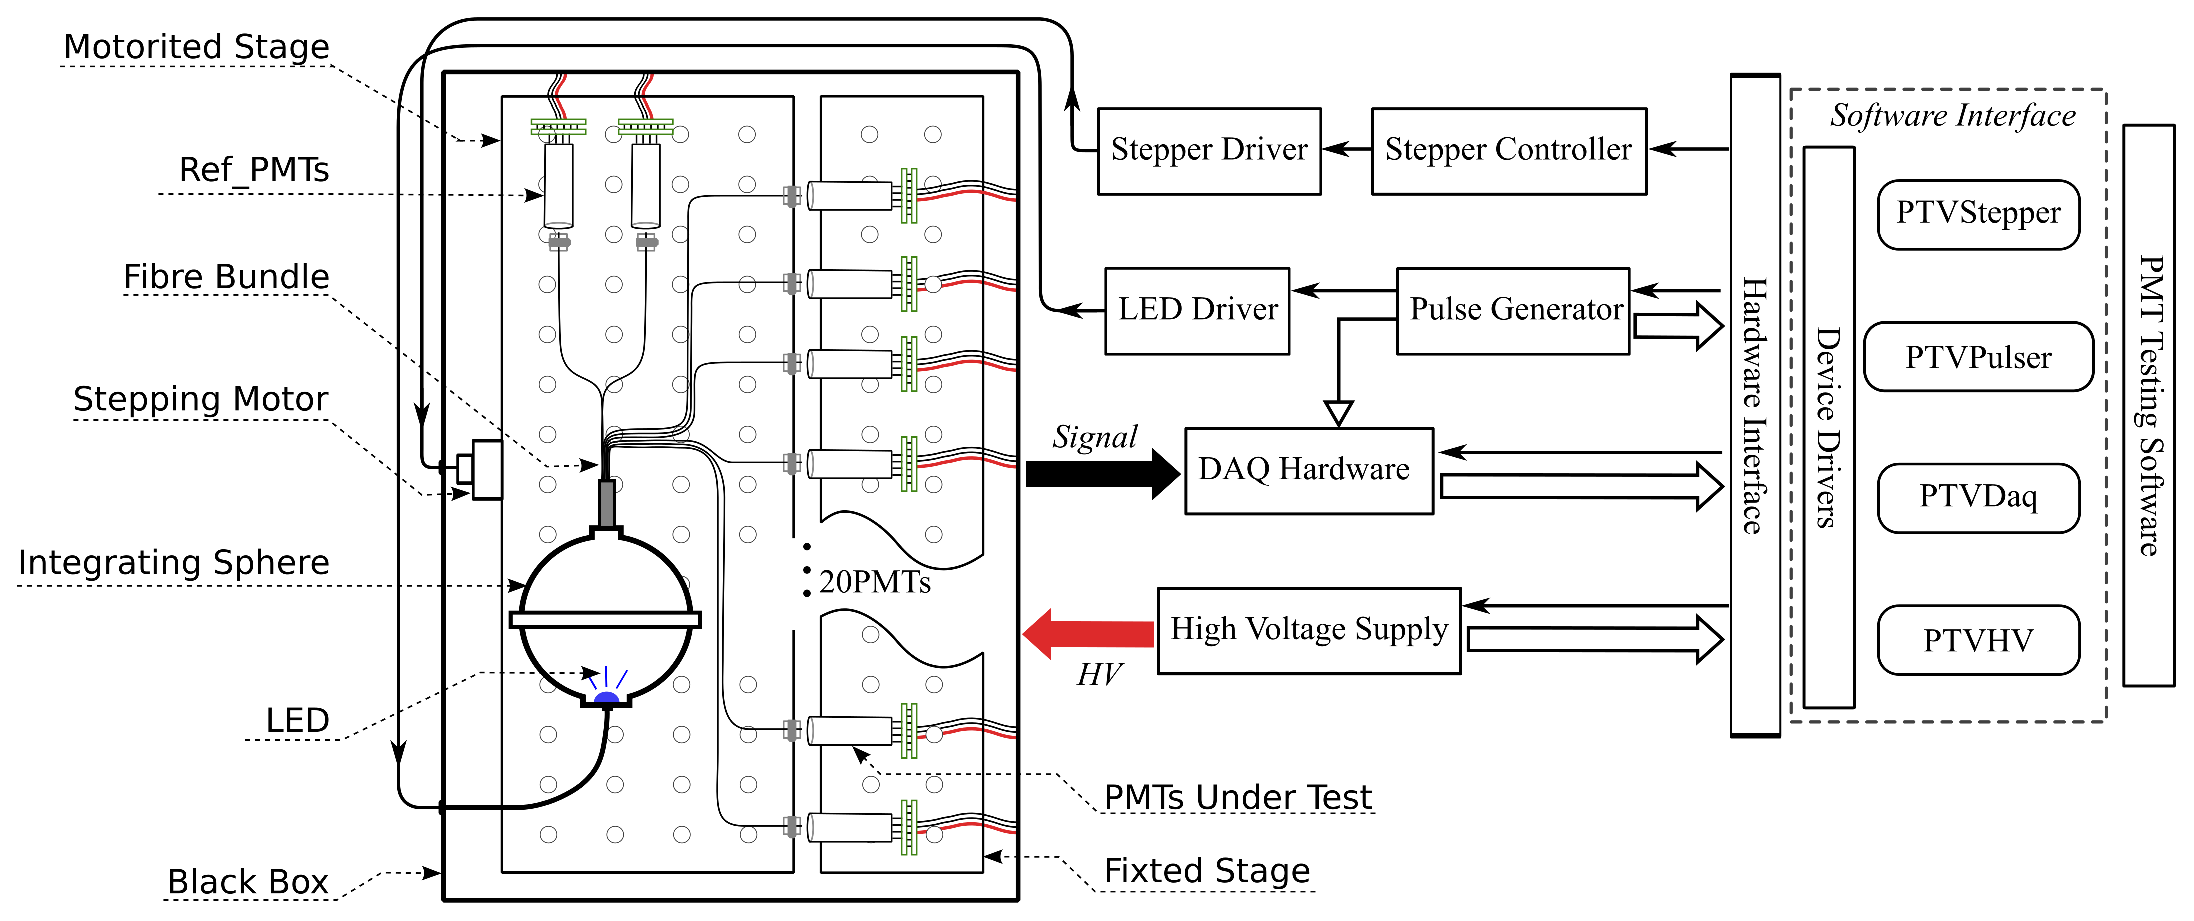
\includegraphics[width=160mm]{testbench_overview}
\caption{Schematic diagram of the PMT test bench system.\textit{PTVStepper}, \textit{PTVPulser}, \textit{PTVDaq} and \textit{PTVHV} are abstract classes which separate the testing software from the hardware implementation details.}
\label{fig:testbench_overveiw}
\end{figure*}

The major design considerations of the test bench is summarized as follows:
\begin{itemize}
 \item \textit{Large capacity}: This is the primary driving force for developping a test bench dedicated for PMT characterization.
 Testing multiple tubes simultaneously can increase the efficiency and save project time tremendously.
 This is a critical factor in large projects such as DAMPE PSD.
 \item \textit{Automation}: A single test run ususally takes several hours, during which most operations are trivial jobs like changing voltage, changing light intensity, starting~/~stopping DAQ.
 Manual operations are inefficient and unreliable in such a long testing period.
 Thus computer controllable hardwares should be used whenever possible and corresponding software should be developped to automate these trivial operations.
 Manual intervention is only expected in the beginning when mounting PMTs and configuring the software and in the end when unmounting PMTs and assessing testing result. 
 \item \textit{Versatility}: As indicated in Sec.\ref{sec:introduction}, the test bench is not designed for single use.
 %It will be utilitized in different experiments with different testing requirements.
 T\-h\-u\-s potential use cases should be considered and appropriate hardwares should be set up in the first place.
 In particular, cathode surface scanning capability is desirable in use cases like PET where several scintillators are coupled to a single PMT. 
 \item \textit{Flexibility}: As a by product of versatiltiy, flexibility is needed both in terms of hardware and software.
 The hardware platform should be extensible and allow complex testing configurations.
 The software should accommodate any changes in the hardware easily, while keeping the high level functionality unchanged and portable. 
\end{itemize}

%%%%%%%%%%%%%%%% Main Text Body %%%%%%%%%%%%%%%%%%%%%%%
\section{Description of the test bench}
\label{sec:description}

A schematic diagram of the final design is shown in Fig.\ref{fig:testbench_overveiw}.
The test bench can test up to 25 PMTs in a single run.
Light pulses are distributed to each tube through an integrating sphere and a fibre bundle, which are mounted on a three-dimensional motorized stage.
PMTs under test will be mounted on a separate fixed stage, thus allowing position scanning of all tubes simultaneously.
Two additional PMTs will be mounted on the motorized stage, serving as reference to monitor the stability of the light source as well as the performance of the whole system(see Sec.\ref{sec:performance}).
They will move with the light distribution system and not be removed from their fixed positions during all test runs. 
Both stages are housed in a light-tight box made of aluminium alloy, with the dimension of $176cm\times100cm\times78cm$.
The box is painted black inside and out and can be opened from the top plate for tube mounting.
All other devices are located outside the light-tight box.
Cables are led out through light-tight cable feedthroughs left in the side plate.
The test bench and all associated devices are sitted in a cleanroom of class 100000, the temperature of which is controlled around 22\textpm2\textcelsius~all the time.

In the following, key components of the test bench will be described in detail.
\subsection{Motorized and Fixed Stages}
\label{sec:stages}

The motorized and fixed stages are the main body of the test bench.
All other objects inside the light-tight box will be mounted on the top of them.
They are arranged face to face with each other and are both covered with an optical breadboard of an area $1560mm\times250mm$, as shown in Fig.\ref{fig:stages}.
The optical breadboards are made of \SI{2.5}{cm} thick stainless steel, which provides substantial resistance to deformation in this application.
The grid pattern of tapped holes on the surface facilitate mounting/unmounting operations, which not only increase efficiency but also provide extra flexibility in testing configuration setup.
In particular, customized fixtures for fibres and tubes have been designed for accurate poistioning.

\begin{figure}[h!]
 \centering
 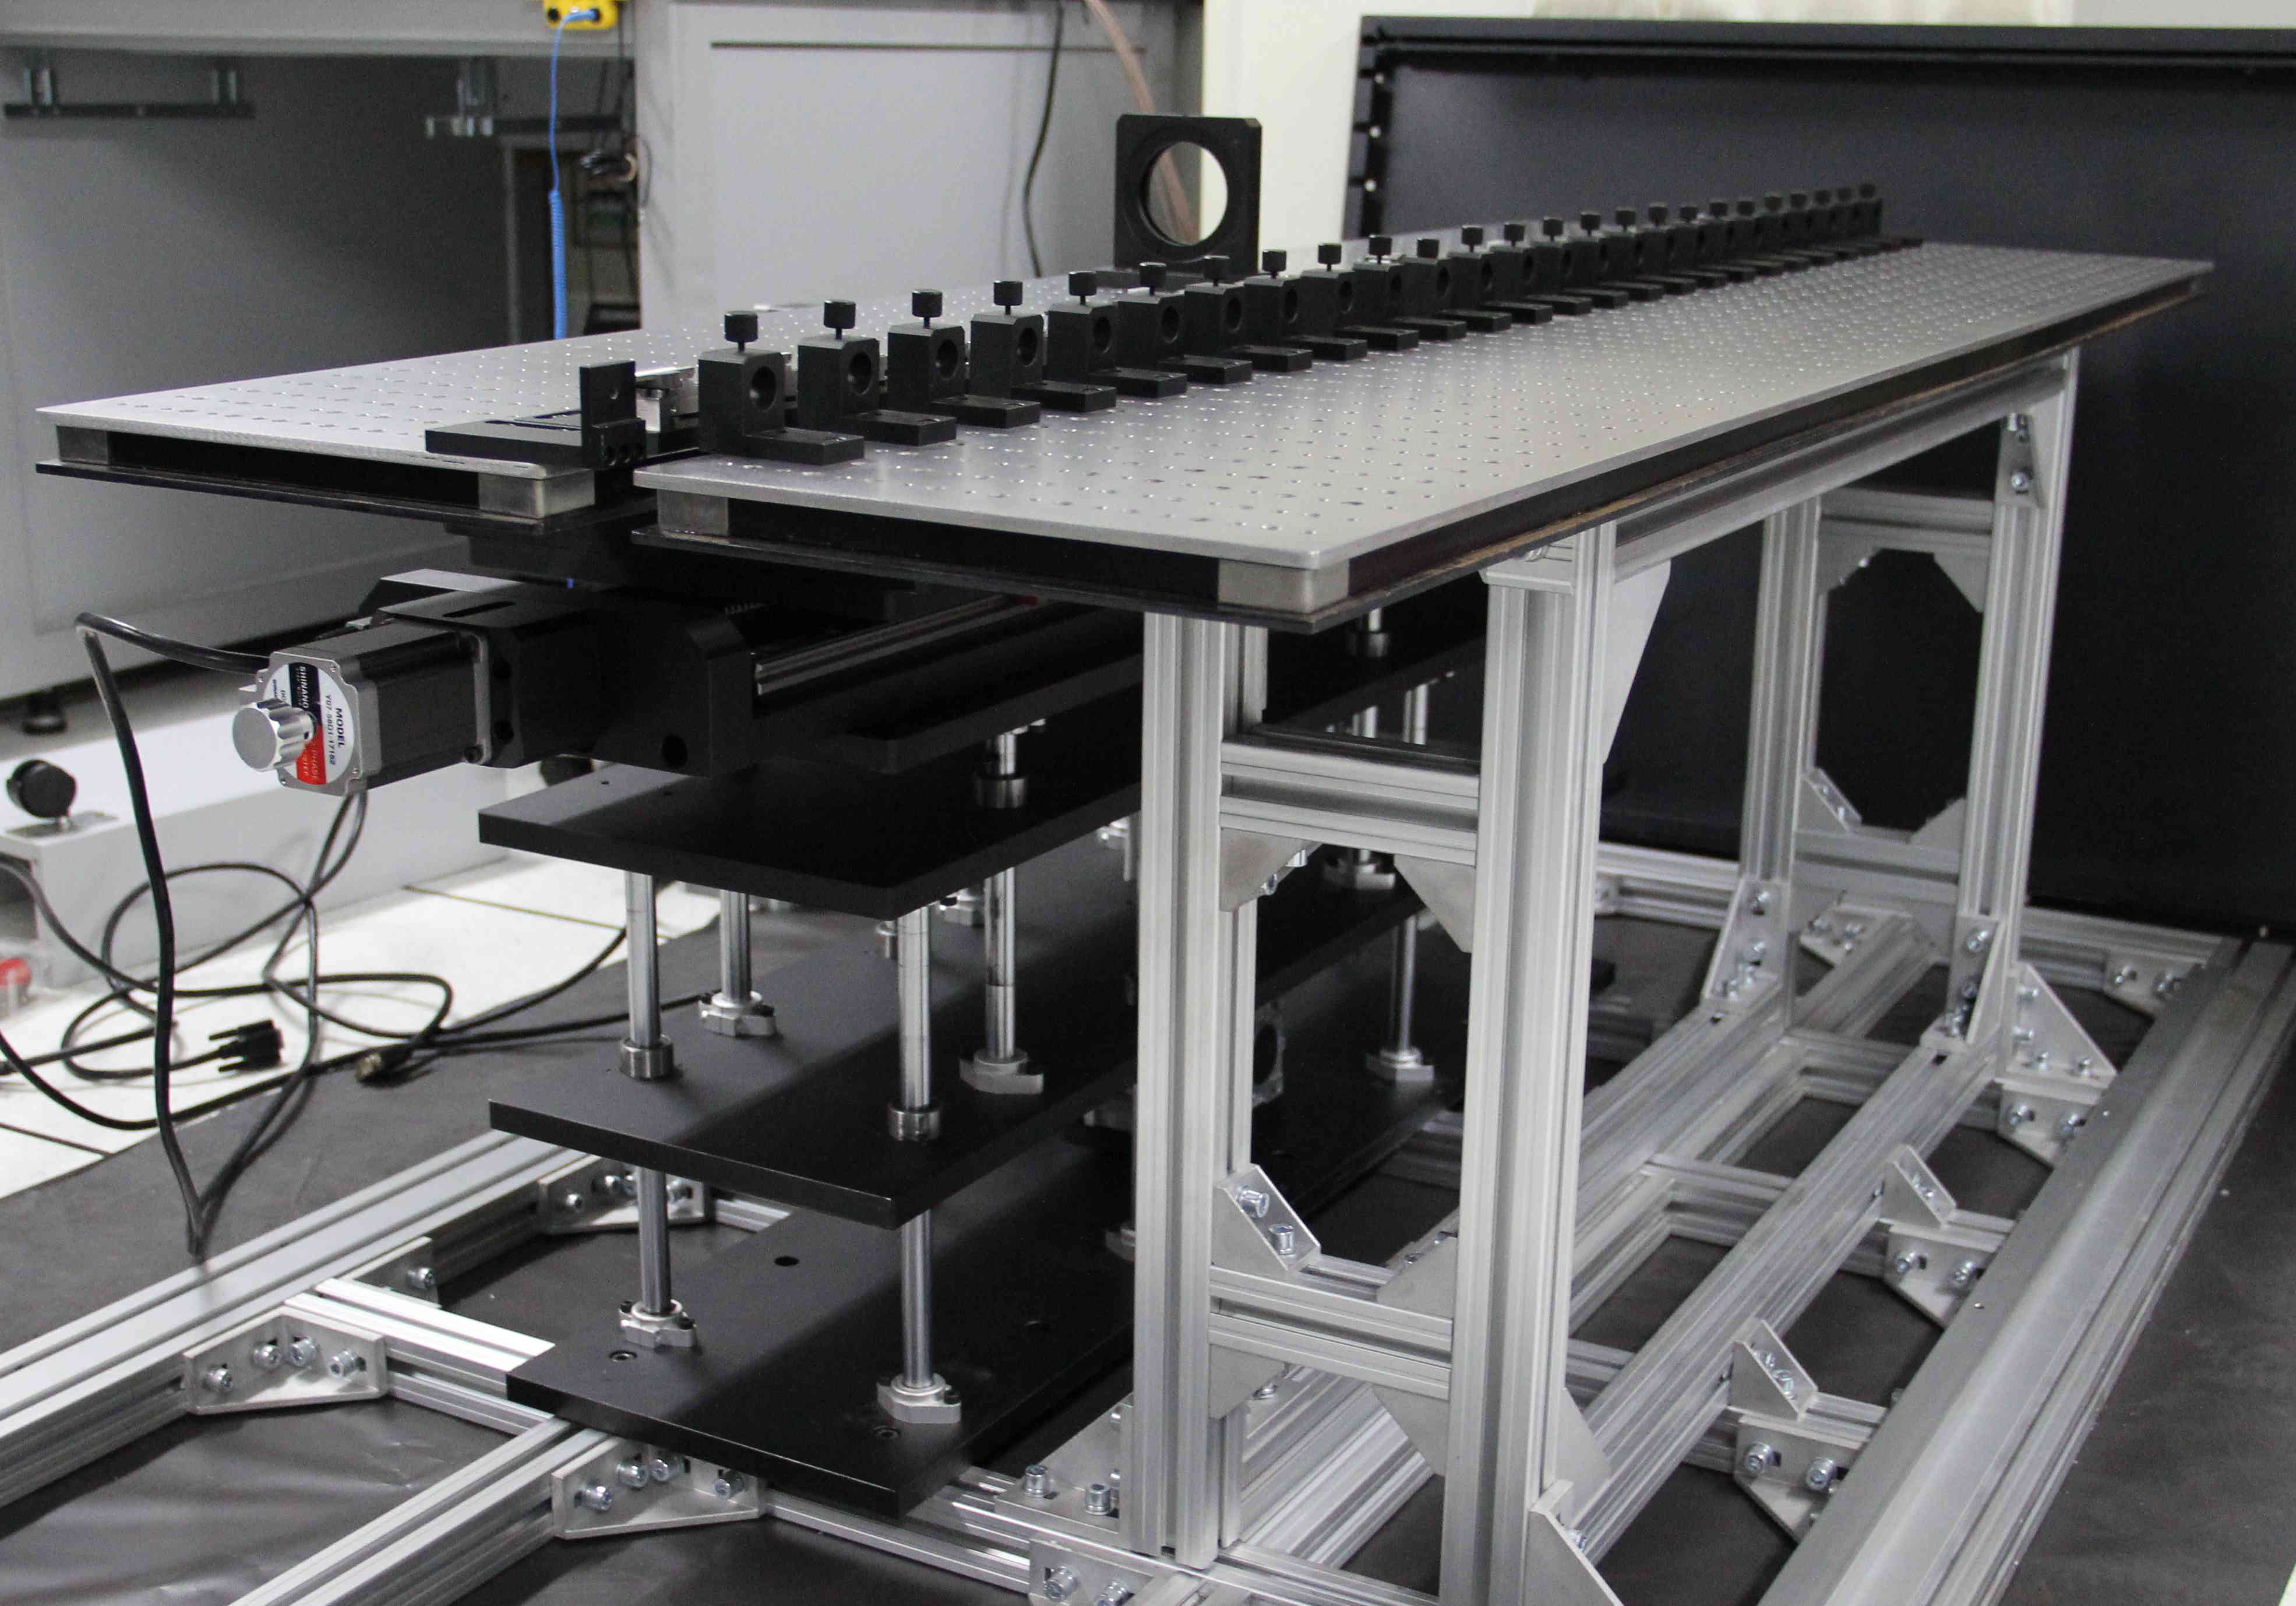
\includegraphics[width=90mm]{stage1_crop}
\caption{Motorized and fixed stages before assembly.}
\label{fig:stages}
\end{figure} 

\begin{figure*}
 \centering
 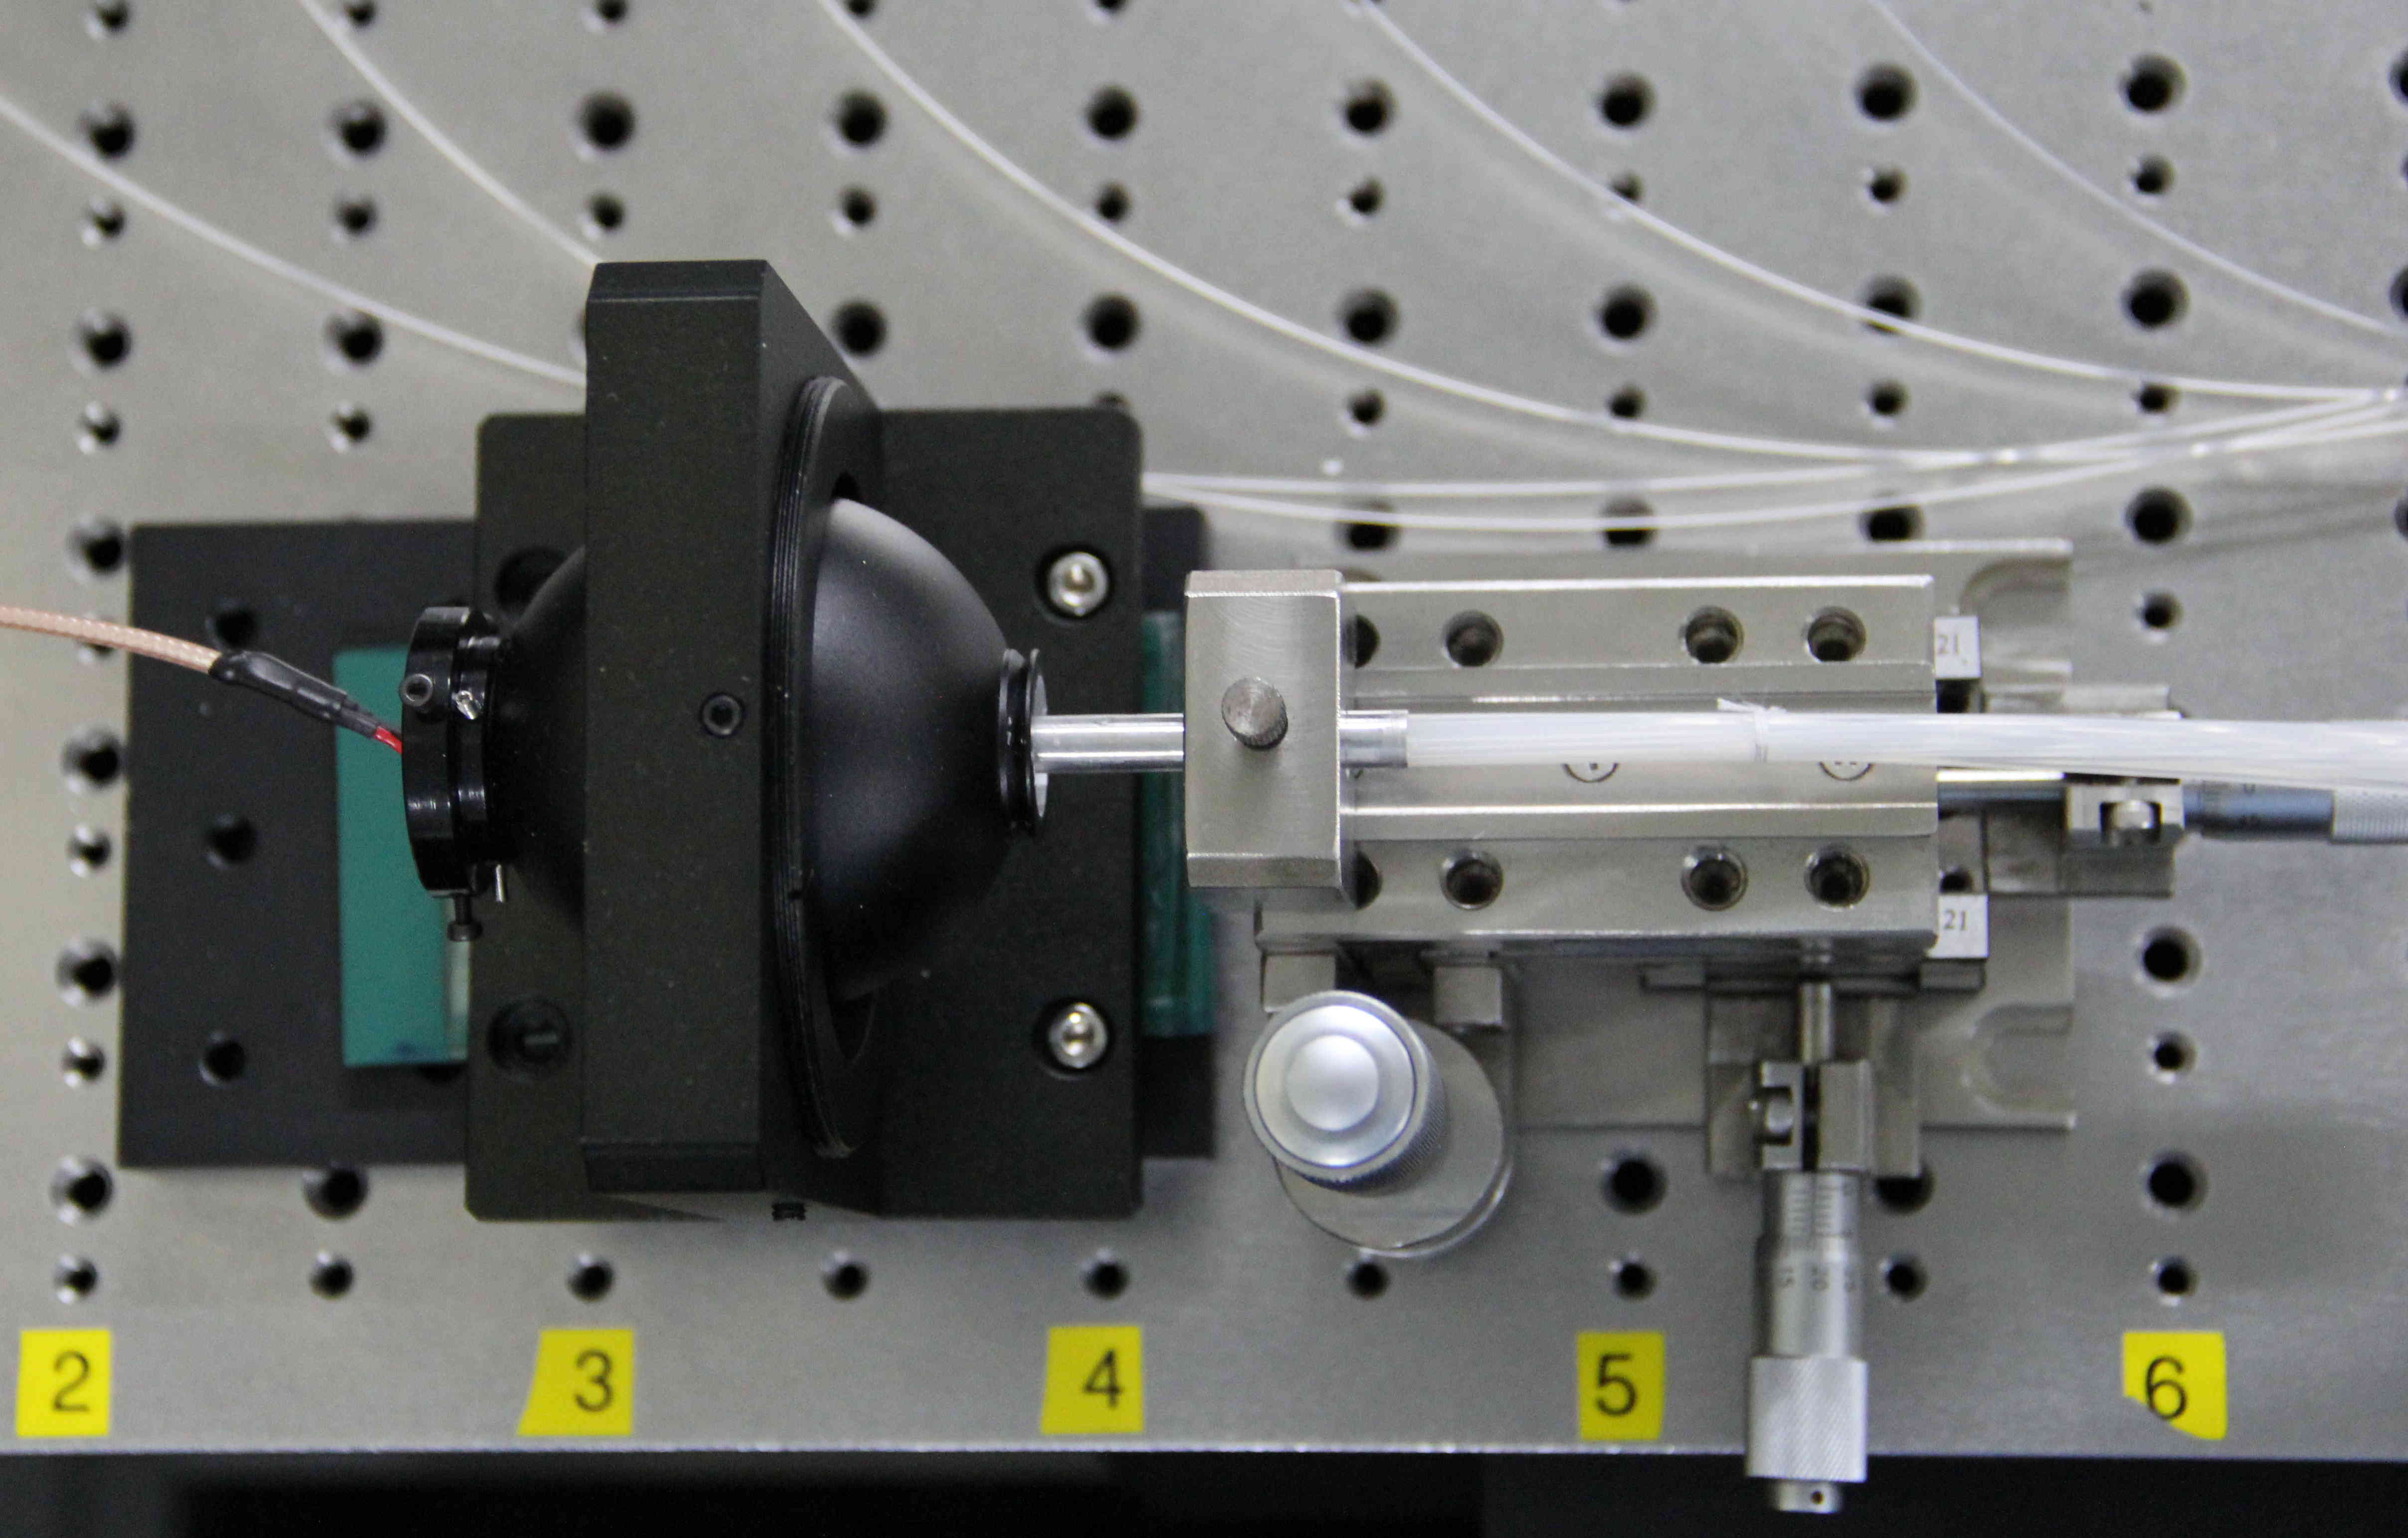
\includegraphics[width=90mm]{light_source1_crop}
\caption{Light source and its distribution system}
\label{fig:light_source}
\end{figure*} 

The load capacity of the motorized stage is \SI{30}{\kilo\gram}, which is sufficient for all use cases.
It is driven by three stepping motors with a minimum step of \SI{1.56}{\micro\meter}.
The travel range in the horizontal direction and vertical direction is \SI{60}{\milli\meter} and \SI{70}{\milli\meter} respectively.
Thus the maximum scanning area is $60mm\times60mm$, which covers the size of the majority of PMTs.
The third direction with a travel range of $15mm$ is added to control the gap between the fibre and the tube's cathode surface.
This may also be useful when extra space is needed for unmounting tubes without disturbing the optical fibres. 
All stepping motors are controlled by a motion controller MPC07SP from Leetro~\cite{leetro}, which possesses a PCI interface for remote control.

\subsection{Light Source}
\label{sec:light_source}

A high-power blue LED~\cite{zlight}(\SI{3}{\watt}, \SIrange{465}{485}{\nano\meter}) coupled to a \SI{5}{\centi\meter} diameter integrating sphere is adoptted as the light source of the test bench.
The LED has been used before successfully in the monitoring and calibration system of Neutron Wall Detector at IMP~\cite{yuyuhong_led} and proved to be suitable for massive light distribution.
The integrating sphere, which is coated interiorly with highly reflective material($\approx$\SI{98}{\percent} at \SI{400}{\nano\meter}), is used to convert the LED into a uniform light source.
To get better heat dissipation, the LED is fixed on a special designed base using thermally conductive silicone rubber and then coupled to the sphere directly making the whole sphere as its heat sink.
The uniformity of the light source has been verified using a Hamamastu R4443 Mod2 PMT read out by the groud test electronics of DAMPE(Sec.\ref{sec:application}). 
The result is shown in Fig.\ref{fig:uniformity_integratingsphere}. 
An uniformity within \textpm\SI{0.5}{\percent} has been reached, which makes the coupling between the light source and fibre bundle much easier and additional calibration for the spatial effect of the light source not needed. 

\begin{figure}[h!]
 \centering
 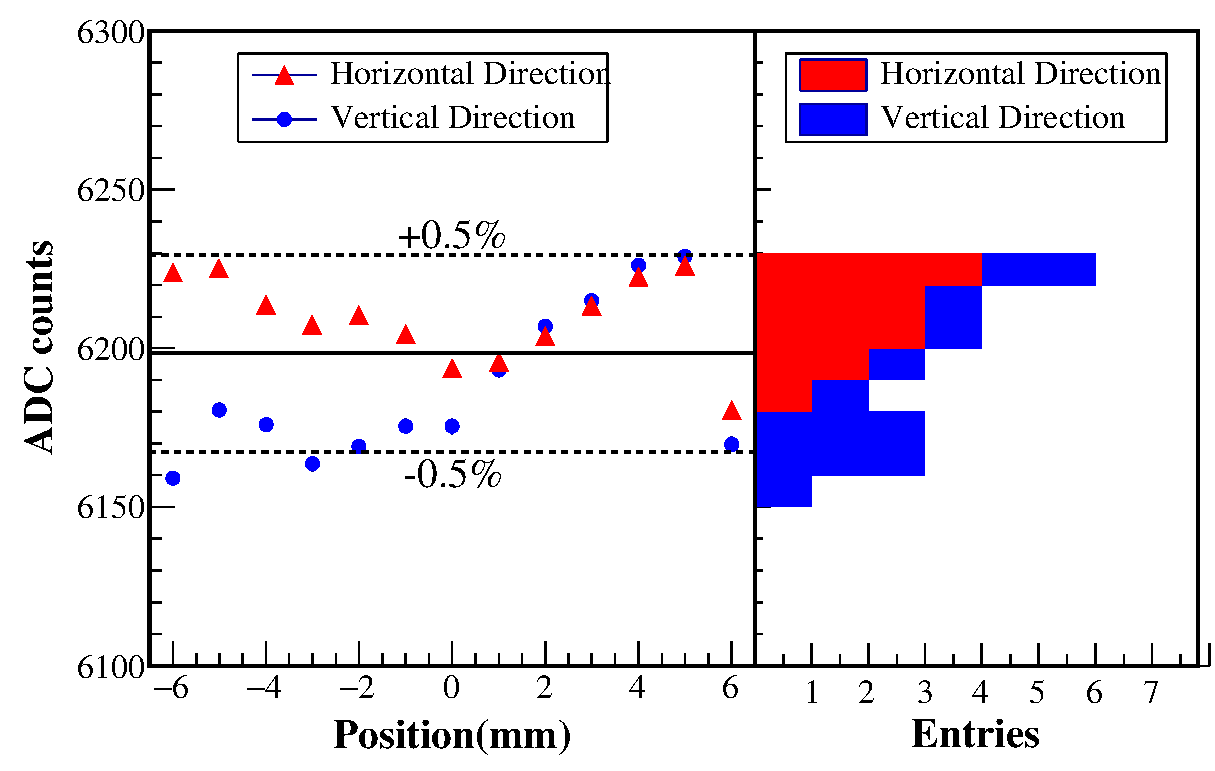
\includegraphics[width=90mm]{uniformity_integratingsphere}
\caption{Spatial uniformity of the integrating sphere.}
\label{fig:uniformity_integratingsphere}
\end{figure} 
  
\begin{figure}[h!]
 \centering
 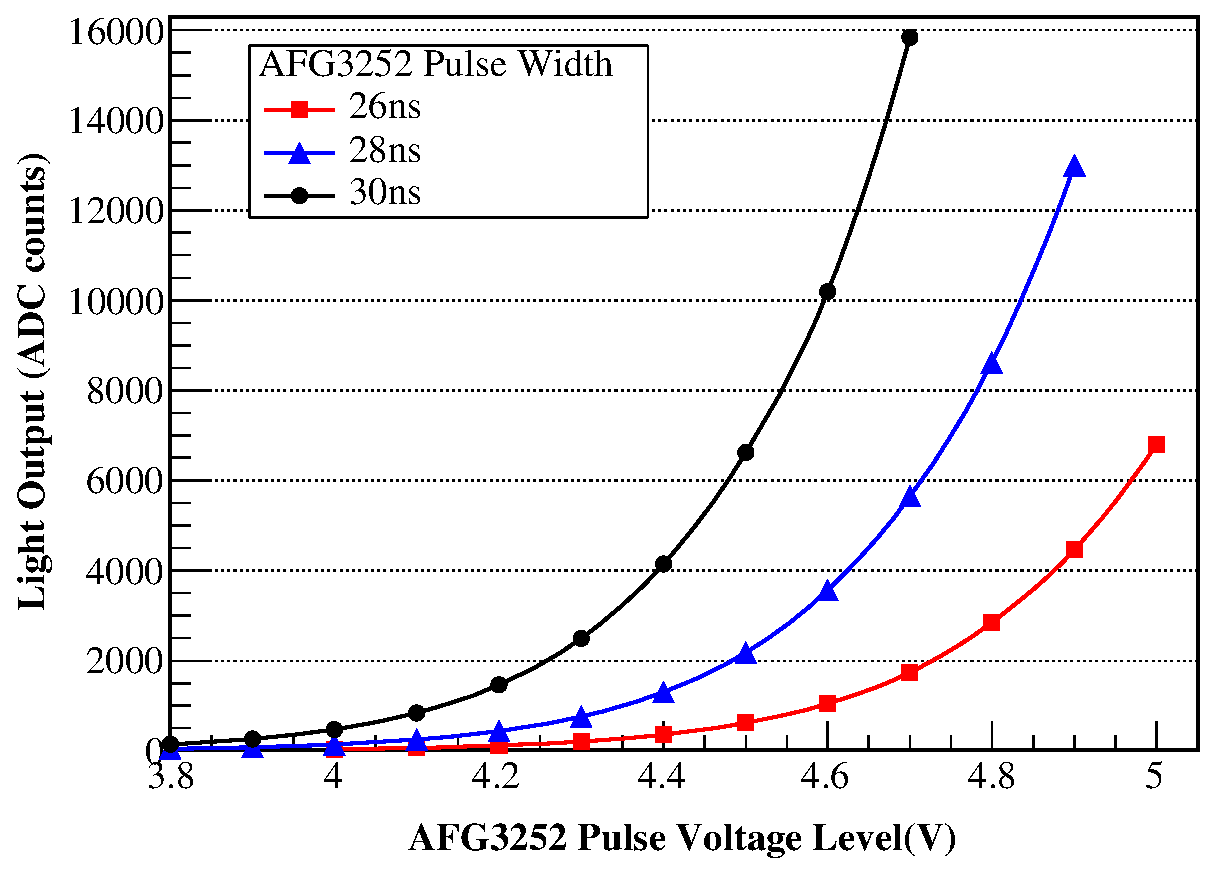
\includegraphics[width=90mm]{intesityVSvoltage}
\caption{Light intensity as a function of AFG3252 pulse voltage}
\label{fig:afg3252_intensityVSvoltage}
\end{figure} 

An off the shelf hardware, Tektronix AFG3252 arbitrary/ function generator, is adpoted as the LED driver.
As a commertial product, it possesses a rich set of interfaces for remote control.
All the pulse parameters of AFG3252 can be adjusted in a wide range with high precison as show in Table \ref{tab:afg3252} and an example is given in Fig.\ref{fig:afg3252_intensityVSvoltage}.
This is a critical feature for a test bench with an objective of versatiltiy, as diverse requirements for the light source exist for different applications.
AFG3252 also has two analog outputs which can be synchronized together.
Thus it be used as a trigger generator at the same time it driving the LED, which will symplify the DAQ configuration in most use cases. 
All these features make it an effective replacement of a dedicated LED driver. 
After all, a stability better than \SI{0.5}{\percent} has been achieved after light intensity correction, the details of which will be given in Sec.\ref{sec:performance}.

\begin{figure}[h]
 \centering
 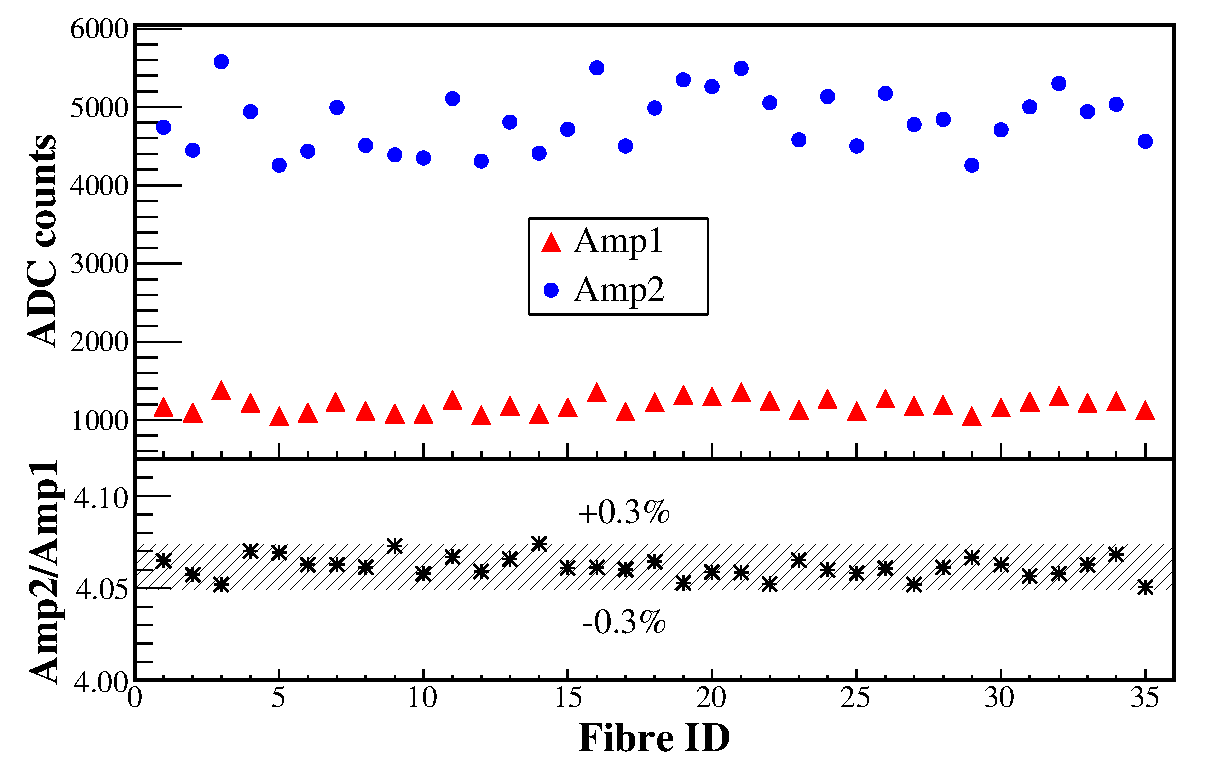
\includegraphics[width=90mm]{fibre_diff}
\caption{Transmission difference of the fibres}
\label{fig:fibre_diff}
\end{figure} 

\begin{figure*}
\centering
 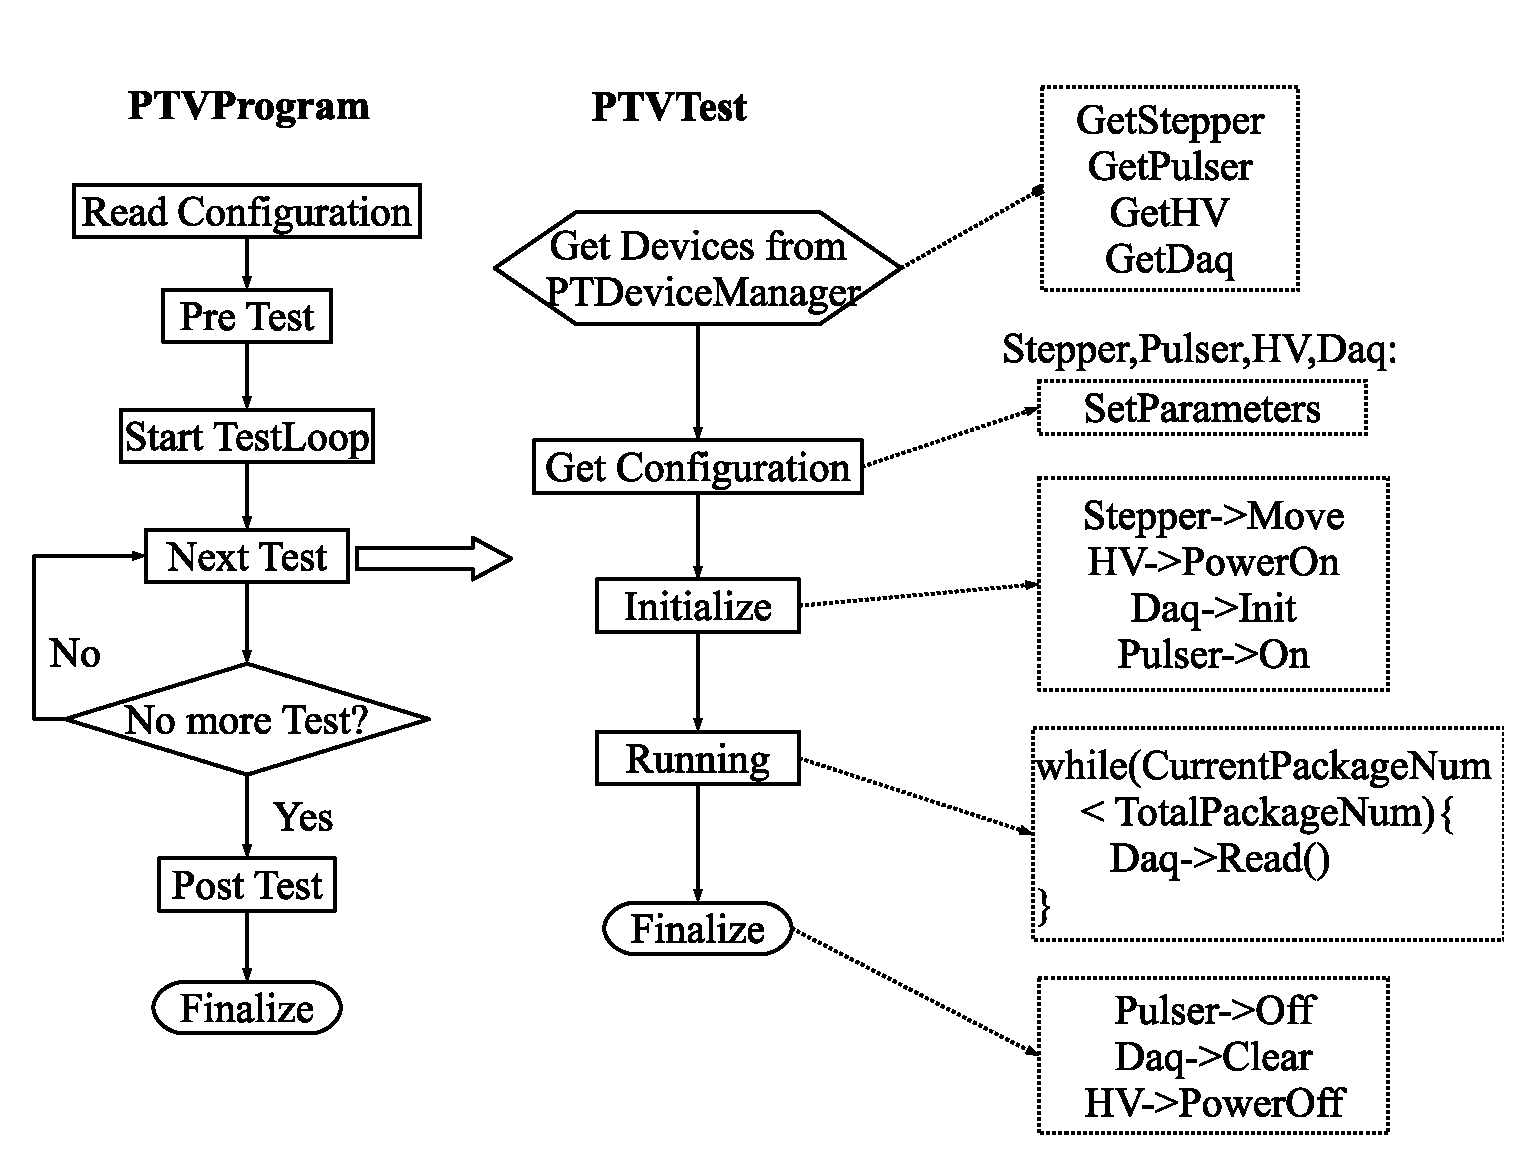
\includegraphics[width=140mm]{software_framework}
\caption{General PMT testing framework}
\label{fig:software_framework}
\end{figure*}

\begin{figure*}[t]
 \centering
 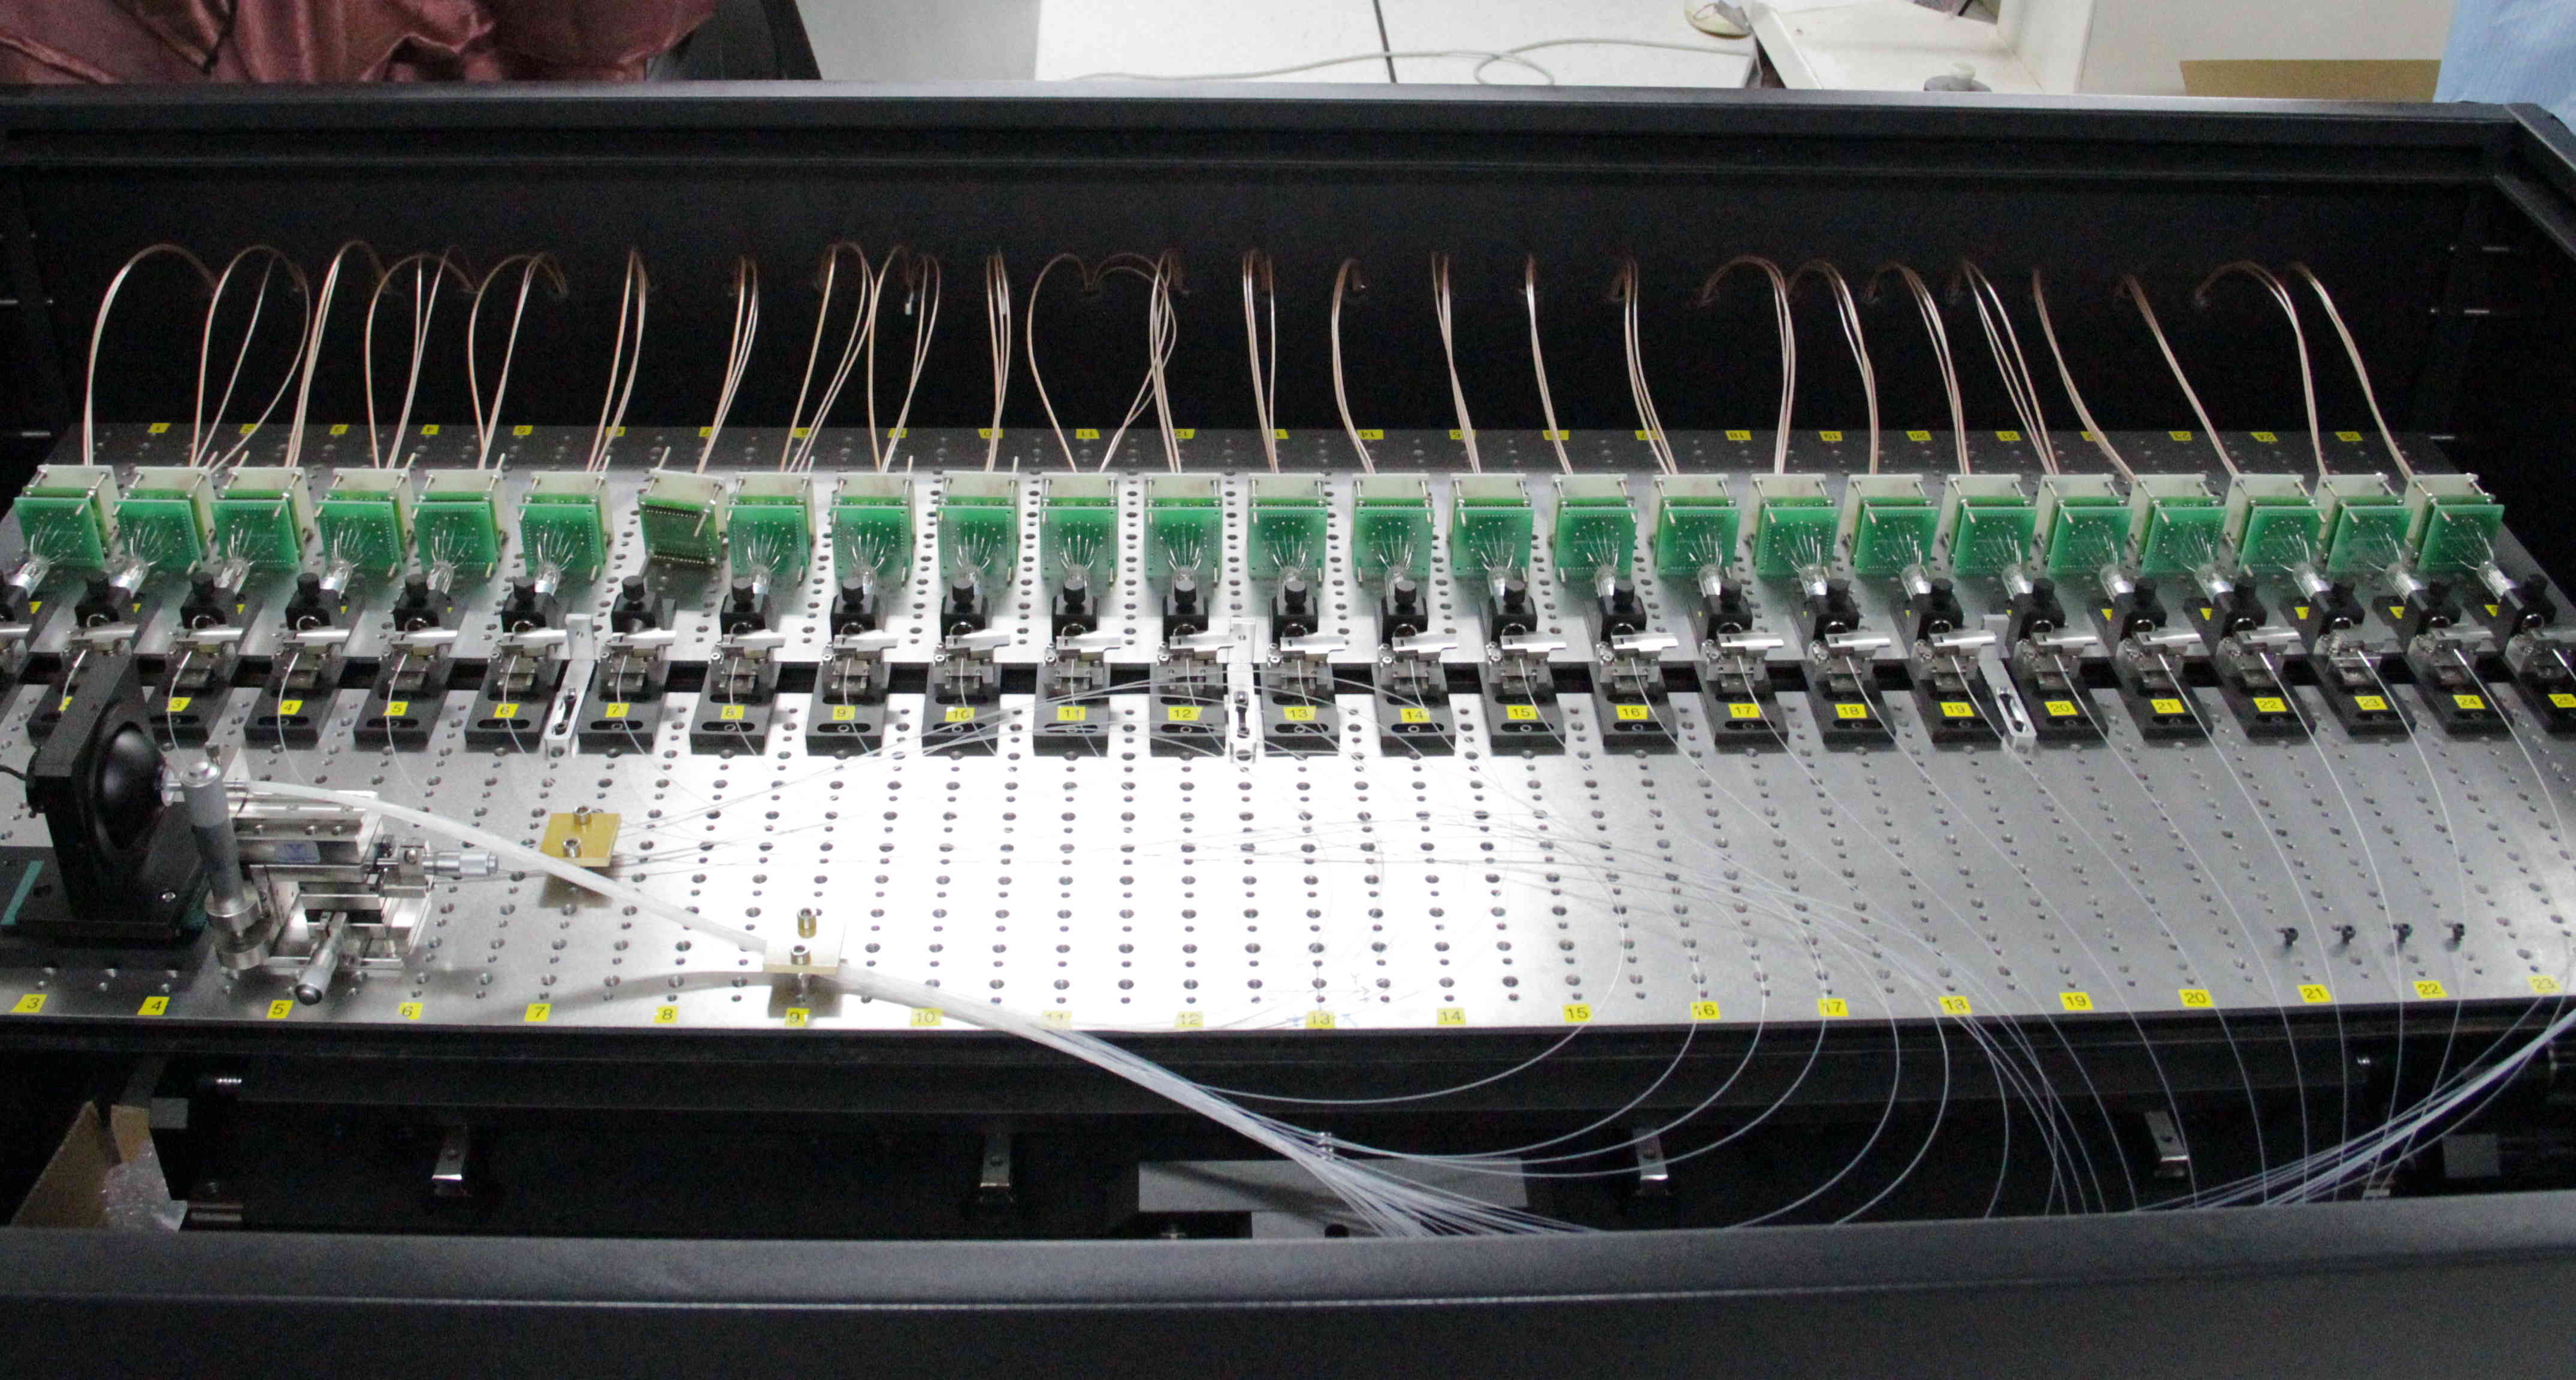
\includegraphics[width=140mm]{integration1_crop}
\caption{The integrated testbench,with tubes under test mounted.}
\label{fig:integrated_testbench}
\end{figure*}

\begin{figure*}
 \centering
 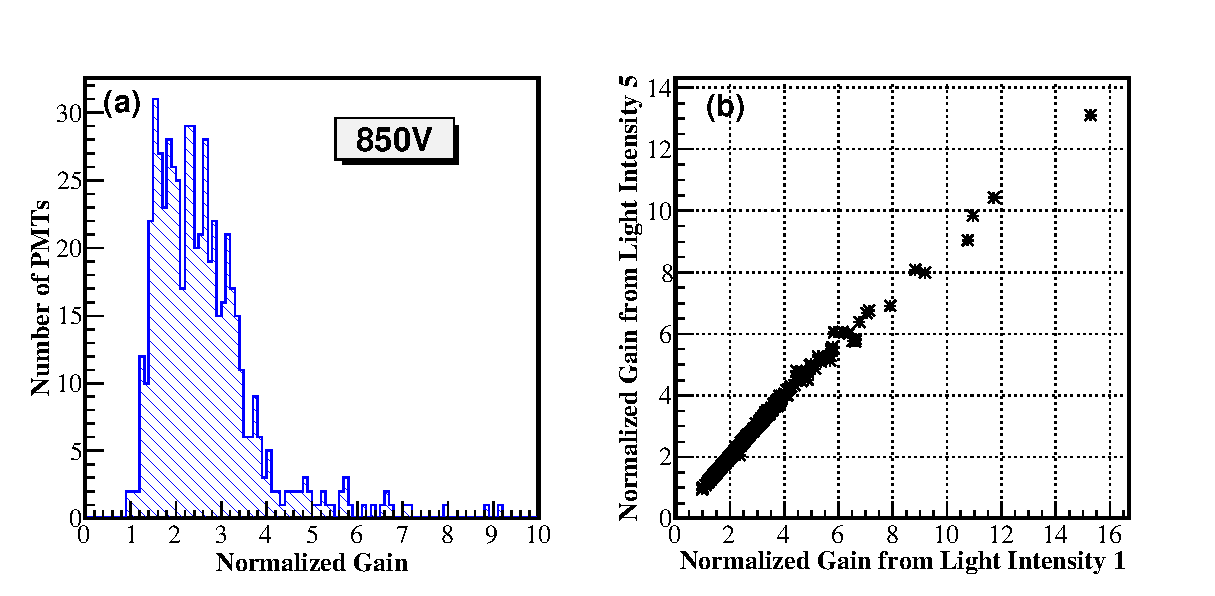
\includegraphics[width=140mm]{GainDist_Correlation}
\caption{Relative Gain Distribution(Normalized to AA2483)}
\label{fig:gain_dist}
\end{figure*}

\begin{table}[h!]
\caption{Summary of AFG3252 Pulse Mode Characteristics}
\label{tab:afg3252}
 \begin{center}
 \begin{tabular}{lr}
 \multicolumn{2}{l}{Summary of AFG3252 pulse mode characteristics}\\ \hline
 Frequecny & max \SI{120}{\MHz} \\
 Amplitude & \SIrange{0}{5}{\volt} \\
           & resolution \SI{0.01}{\volt} \\
 Pulse width & min \SI{4}{\nano\second} \\
             & resolution \SI{10}{\pico\second} \\
 Leading edge & \SI{2.5}{\nano\second} to 0.625*pusle period \\
 Trailing edge & \SI{2.5}{\nano\second} to 0.625*pusle period \\
 %Jitter(typical) & \SI{100}{\pico\second} \\
 Interface     & GPIB, LAN, USB
 \end{tabular}
 \end{center}
\end{table} 

\begin{comment}
One limitation of AFG3252 is that it has a limited leading edge of \SI{2.5}{ns}.
This may not be suitable for timing-related characterizations, where ultra-short(down to hundreds of \si{\pico\second} magnitude) light pulse is preferred.
In this case, a dedicated LED driver of special design(commertial or home-made)shall be used instead.
However the rich interfaces AFG3252 possesses still make it valuable as a trigger generator to control both the LED driver and DAQ remotely. 
\end{comment}

\subsection{Fibre Bundle}
\label{sec:fibre_bundle}

A bundle of 35(25 for test, 2 for reference and 13 spares) plastic clad silica fibres is utilized to distribute light to each PMT under test.
The fibres are \SI{1.5}{\meter} long and have a \SI{400}{\micro\meter} diameter core and a \SI{550}{\micro\meter} diameter cladding.
The numerical aperture(NA) is 0.37.
The relatively large core and large NA make the fibre an efficient light extracter of integrating sphere output. 
For easier manipulation and to protect the fibres from mechanical stress, both ends of the fibre bundle are coated with stainless steel ferrules.
The bundle end is coupled to the centre of the output port of integrating sphere using a stable fibre alignment stage.
On the other end, each fibre is fixed using a customized fibre holder which allows two-dimensional position adjustment.
In each test run, all used fibres will aligned to the centre of their corresponding PMT's input window with a precision of \SI{0.5}{\milli\meter}.  

After coupling to the integrating sphere, the light output of each fibre is measured and a variance of \SI{10}{\percent} is observed among the fibres. 
As the un-uniformity of the light source(see Sec.\ref{sec:light_source}) is much less than the mesurement result, the result is a direct reflection of the transmition difference among the fibres.
Plus, the result also shows no dependency on the light intesity used(see Fig.\ref{fig:fibre_diff}). 
This is within expectation, because transmition coefficient is an intrinsic characteristic of the fibre itself.
The transmition difference got here will be used later in the relative gain measurement,see Sec.\ref{sec:psd_gain}.
%%The testing configuration includes two R4443 Mode PMTs, one for light source monitoring and the other one for fibre testing.
%%As stable fixture for the tubes and fibres are utilitized, the major uncertainty comes from the coupling distance between the fibre and the PMT in the longitudinal direction.


\subsection{Electronics and High Voltage Supply}
\label{sec:electronics}

\begin{comment}
To get more realistic results, electronics for PSD ground test is utilitized for the PMT test.
It consists of a front end electronics(FEE) box and a data acquisition(DAQ) board.
Both of them are standalone devices powered by a standalone DC power.
The FEE is based on the same design as the flight model of PSD, except that it uses commertial grade components instead.

Signals from R4443-Mod2 are connected to the FEE box directly and undergo charge integration and pusle shaping there.
Trigger signal from AFG3252 is connected to the DAQ board, which then dispatch the trigger to the FEE box.
Upon recieving the trigger, FEE will hold and digitize the shaped signal and transmit the digits to the DAQ board for packaging.
The packaged data are finally readout by a computer through the USB port on the DAQ board.
Commands from computer are sent to the DAQ board through a RS232 serial port.
Both the USB and serial interface are controlled using the NI-VISA library.
\end{comment}

A CAMAC system based on Wiener CC-USB control board has been set up for data acquisition.
This system is ready to use and shall be adequate for fast PMT characterization in daily use.
However, it shall be noted that the DAQ system of the test bench is expected to change frequently, as customized electronics with different control interface may be preferred in some project.

A mainframe from CAEN, SY1527LC, is adoptted as the high voltage supply system of the test bench.
While HV boards of various properties can be housed in SY1527LC, the same control interface will be used for all kinds of operation.
This feature simplifies our implementation of the test bench as a versatile equipment.More information about SY1527LC can be found in~\cite{sy1527lc}.

\subsection{Software}
\label{sec:software}

The software system is a critical part of the test bench.
It is developped under Windows in C++ and divided into three hierarchies as follows:
\begin{enumerate}
 \item \textit{Device abstraction}, which not only serves as an interface to the underlying hardwares, but also handles the abstraction of different types of devices. 
 %which serves as an interface to the underlying hardwares.
 \item \textit{Framework libraries}, which defines a general testing pecedure and provides utility classes for configuration and management.
 \item \textit{User inerface}, which provides command line based or graphical executables for user interaction. 
\end{enumerate}

%Designed as a versatile equipment, different hardware modules may be used in the future.
Instead of developping a dedicated program each time a hardware changes, an abstraction of the devices is adoptted to separate the testing procedure from hardware implementation details. 
Abstract classes are defined for four frequently used devices in the test bench, i.e. motion controller, pulse generator, DAQ system and HV supplier, as shown in rounded boxes in Fig.\ref{fig:testbench_overveiw}.
%Common operations of each type of device are extracted as the interface of the corresponding abstract class.
New device only needs to inherit from its corresponding abstract class and implement its interface methods and then registered in the singlton class \textit{PTDeviceManager}, leaving all other part of the software unchanged.
Currently, concrete device classes for the hardware described in Sec.\ref{sec:description} have all been implemented and fully tested.
%Used concrete device class shall be registered in the singlton class \textit{PTDeviceManager} and retrieved from it in other part of the software. 

Built upon the abstract device inerface, a general testing framework is defined as shown in Fig.\ref{fig:software_framework}.
%As a first step, all used concrete device classes shall be registered in the singlton class \textit{PTDeviceManager}.
%Devices are then retrieved from \textit{PTDeviceManager} in all other part of the software.
%Testing procedures are grouped as shown in Fig.\ref{fig:software_framework}.
A \textit{PTVProgram} represents the measurement for a specific characteristic of PMT, such as cathode uniformity, gain and so on.
\textit{PTVTest} is a subunit of \textit{PTVProgram}, which encapsulates the real device operations performed under a specific condition.
%As an example, typical implementation for \textit{PTVTest} using fake code is presented in the third column of Fig.\ref{fig:software_framework}.
Usually, a \textit{PTVProgram} consists of a series of \textit{PTVTest}s, which are invoked sequentially in a test loop.
For example, in cathode uniformity test, the stepping motor will move to a series of positions and the PMT response will be recorded by the DAQ system at each position.
Here, device operations performed at each position constitute a \textit{PTVTest} and tests at all positions constitute a \textit{PTVProgram}.
Additional actions may be added in the \textit{PreTest} and \textit{PostTest} methods of \textit{PTVProgram}, which will be invoked before and after the test loop repectively.
Typically, PMT warming shall be performed in \textit{PreTest} and analysis code shall be added in \textit{PostTest}.
\textit{PTVProgram}s of various testing objectives will finally be chained together to constitute a complete characterization of PMT.

Finally, a light-weight user interface based on PDCurses~\cite{pdcurses} has been developped.
This program features in device control, status monitoring and information logging.
Thanks to the abstraction described above, the architecture of the program is rather independent of the specific hardware used and testing program performed.
A decoding function from binary file to root file~\cite{root} is also incorporated into it for online monitoring.
However, more detailed analysis are considered project specific and not included in the program. 

\section{Application in the PMT testing for PSD of DAMPE}
\label{sec:application}

PSD adopts Hamamastu R4443 Mod2 for scintillation light detection. 
Both dynode5 and dynode8 of R4443 Mod2 are readout by a customized voltage divider to cover the large dynamic range required by PSD.
Signals are then processed by a highly-sensitive ASIC chip(VA160~\cite{va160}) with a linear range of \SIrange{0}{12}{\pico\coulomb} and digitized by an ADC with 14~bits resolution.
Both the gain of dynode8 and the ratio between dynode8 and dynode5 need to be ajusted carefully to accommodate the input range of VA160 and also to keep an uniform response across the whole detector.

General purpose QDC of CAMAC or VME features an input range of several hundreds \SI{}{\pico\coulomb} and thus not suitable for PMT characterization in this application.
Instead, the groud test electronics of DAMPE are utilitized, which is based on the same design as the flight model except that commertial grade components are used.
A dedicated \textit{PTVDaq} has been implemented for this system.

About 20 tubes were tested in a single test run, as shown in Fig.\ref{fig:integrated_testbench}.
A typical test run lasts about 5 hours including 2 hour's PMT warming time before test.
Totally, 28 test runs are performed in a period of about one month.
570 rare R4443 Mod2 tubes are charaterized and 196 of them are selected for production and qualification.
Selection of tubes based the testing data is not the object of this article.
Here, only the major results are presented with a focus on the demonstration of the validity of the test bench. 

\subsection{Testing of Gain of Dynode 8}
\label{sec:psd_gain}

\begin{figure}[h!]
 \centering
 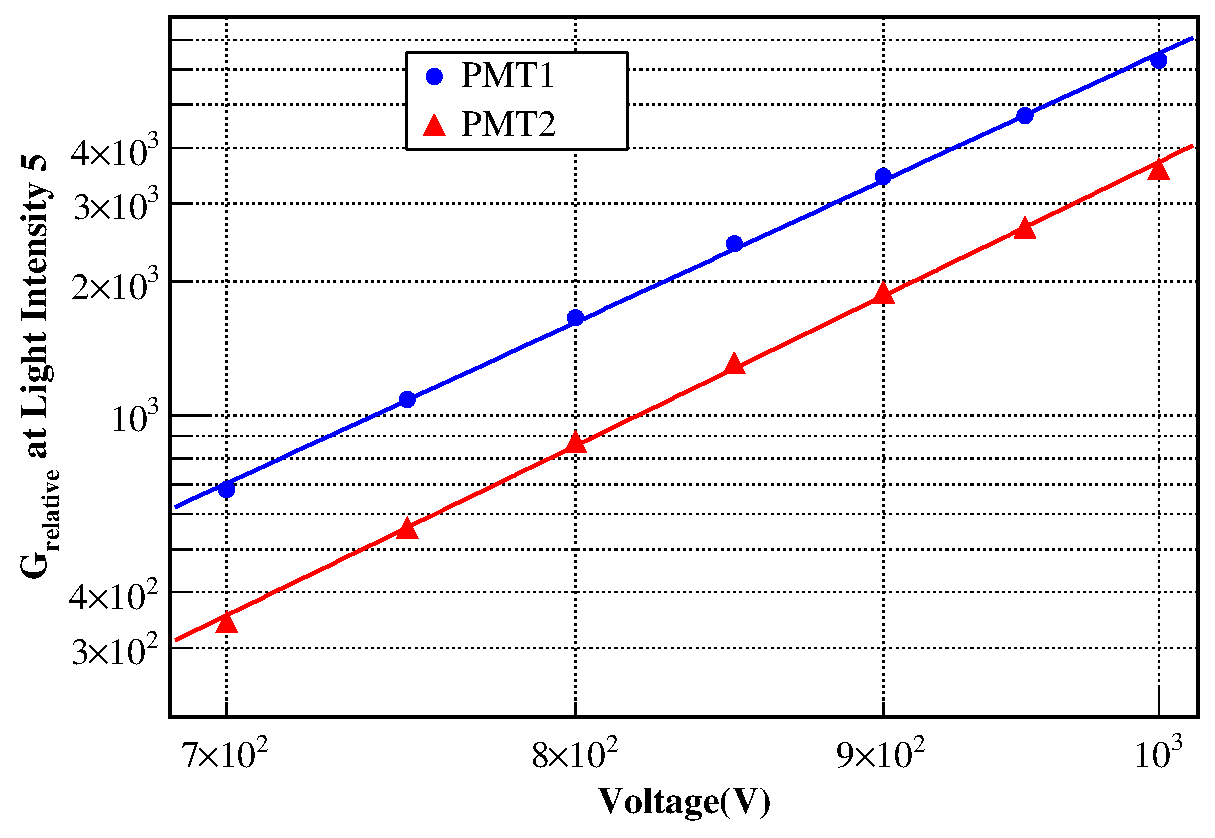
\includegraphics[width=90mm]{gainVSvoltage}
\caption{Gain dependency on high voltage of two PMTs}
\label{fig:gainVSvoltage}
\end{figure} 

\begin{figure}[h!]
 \centering
 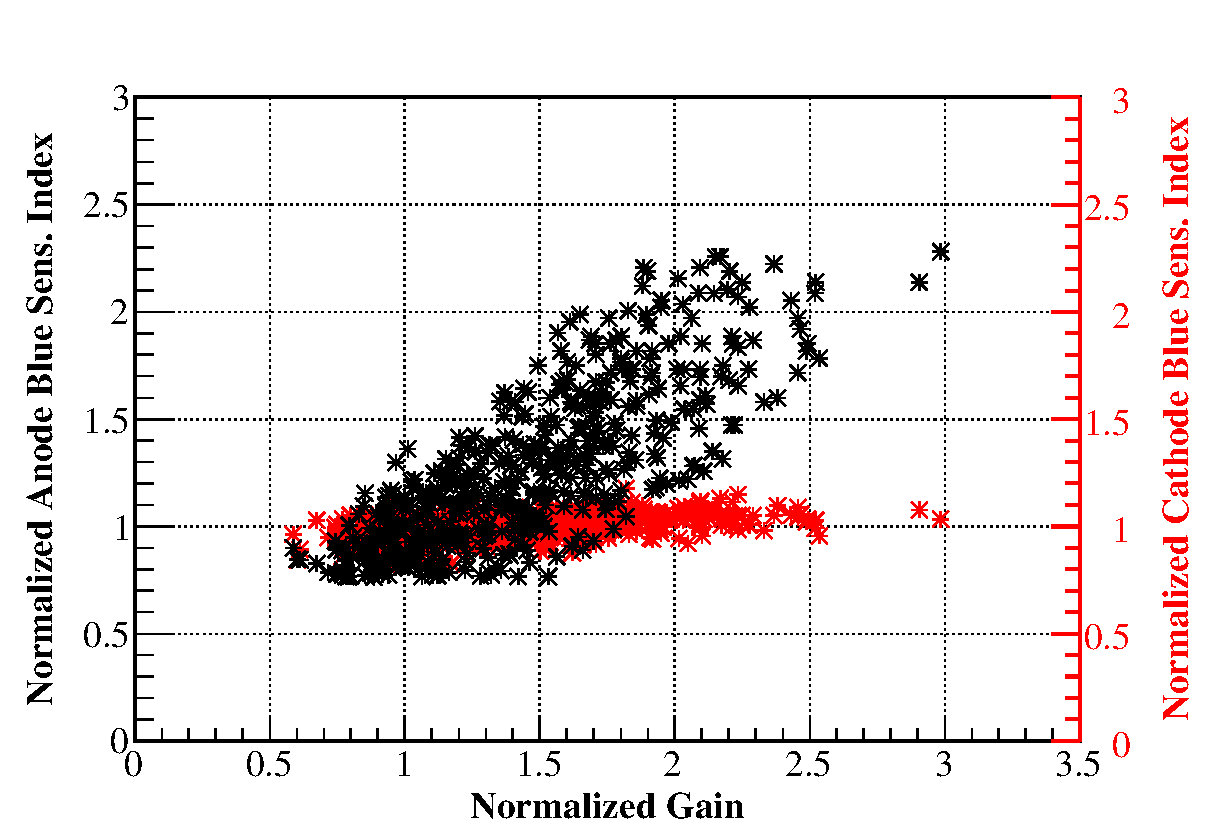
\includegraphics[width=90mm]{correlation}
\caption{Correlation between the parameters given by Hamamastu and the gain tested in this paper}
\label{fig:gain_correlation}
\end{figure} 

The gain of dynode 8 is measured by recording the response of PMT at a fixed light source setting. 
This is a relative method and the result depends on the light intensity:
\begin{equation}
 G_{relative} = L_i \times G(V) = L_i k V^\beta
\end{equation}
where $G(V)$ is the absolute gain of PMT and $L_i$ is the light intensity used.
$G_{relative}$ is a direct reflection of $G(V)$ if the inconsistency of light intensity can be eliminated.
Two corrections are made to accomplish this goal, as follows: 
\begin{equation}
 G_{relative} = \frac{A_{mean}}{K_{runid} T_{chid}}
\end{equation} 
where $A_{mean}$ is the mean value of the raw ADC spectrum at the specified light source setting,
$K_{runid}$ is the light intensity fluctuation of LED between different test runs and $T_{chid}$ is the light transmition difference among testing channels.
$K_{runid}$ can be calculated at each test run using the fixed reference PMT.
$T_{chid}$ mainly comes from the fibres and is a fixed parameter, which has been measured accurately before(Sec.\ref{sec:fibre_bundle}).
These corrections are made for all testing results.

5 light source settings, with a maximum intesity difference of about 2 times, have been used for gain measurement.
The results from different light intensities are cross checked and they are consistent with each other.
Distribution of the relative gain at 850V are shown in (a) of Fig.\ref{fig:gain_dist} and the matching between two light intensities are shown in (b).
7 voltage steps(from 700V to 1000V with a 50V step) are scanned to measure the gain variation as a function of supply voltage.
The results are then fitted using power law function,as shown in Fig.\ref{fig:gainVSvoltage}.

Based on the fitting result,the gain at the Hamamastu equivalent voltage is calculated for comparison with the parameters provided by Hamamastu.
Hamamastu equivalent voltage is the voltage that should be applied to the PSD voltage divider so that the same value on dynode 8 can be achieved as that used by Hamamastu for PMT testing.
Linear correlation between the calculated gain and the anode blue sensitivity index has been observed(Fig.\ref{fig:gain_correlation}).
This is a demonstration of the validity of our testing method.

\subsection{Testing of the Ratio between Dynode8 and Dynode5}
\label{sec:psd_dy58}

\begin{figure}[h]
 \centering
 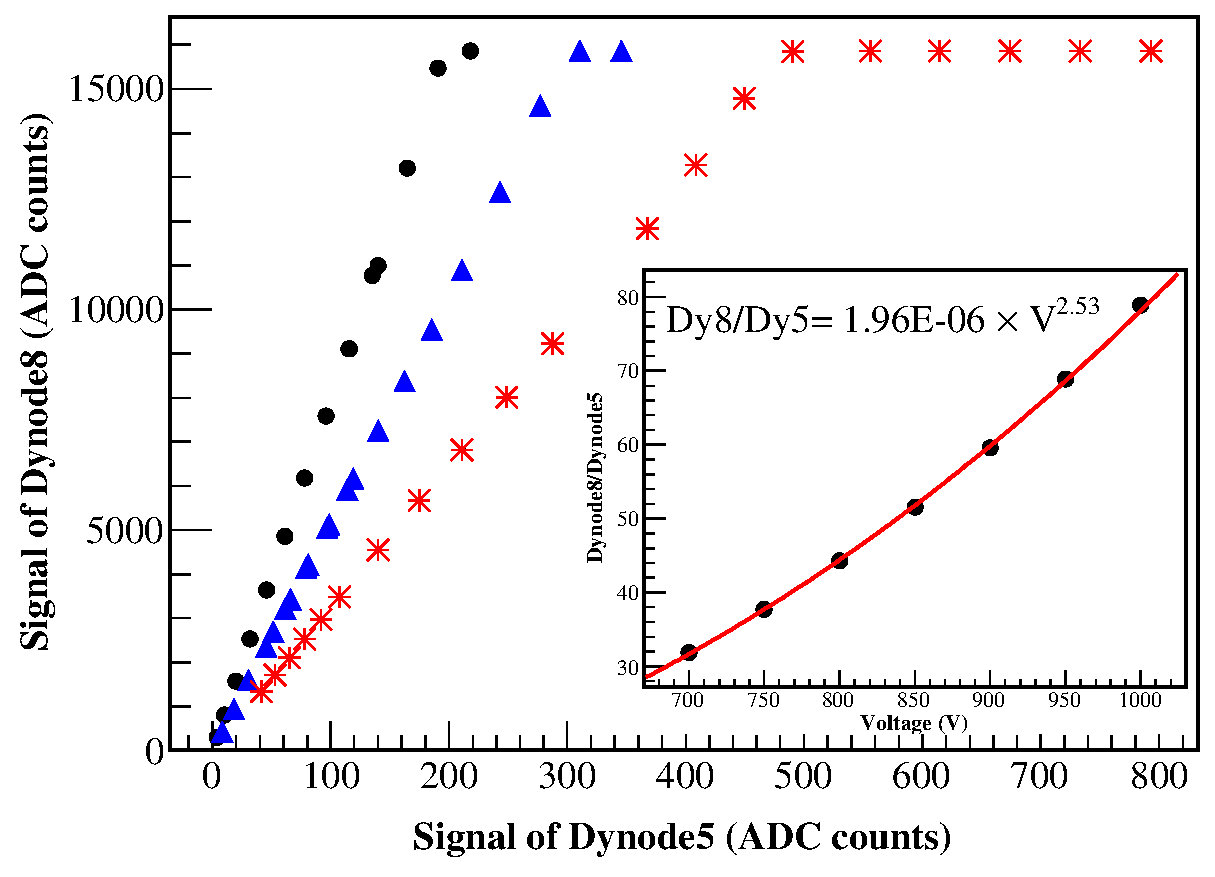
\includegraphics[width=90mm]{dy58_example}
\caption{Example of the Dynode8/Dynode5}
\label{fig:dy58_example}
\end{figure} 

\begin{figure}[h]
 \centering
 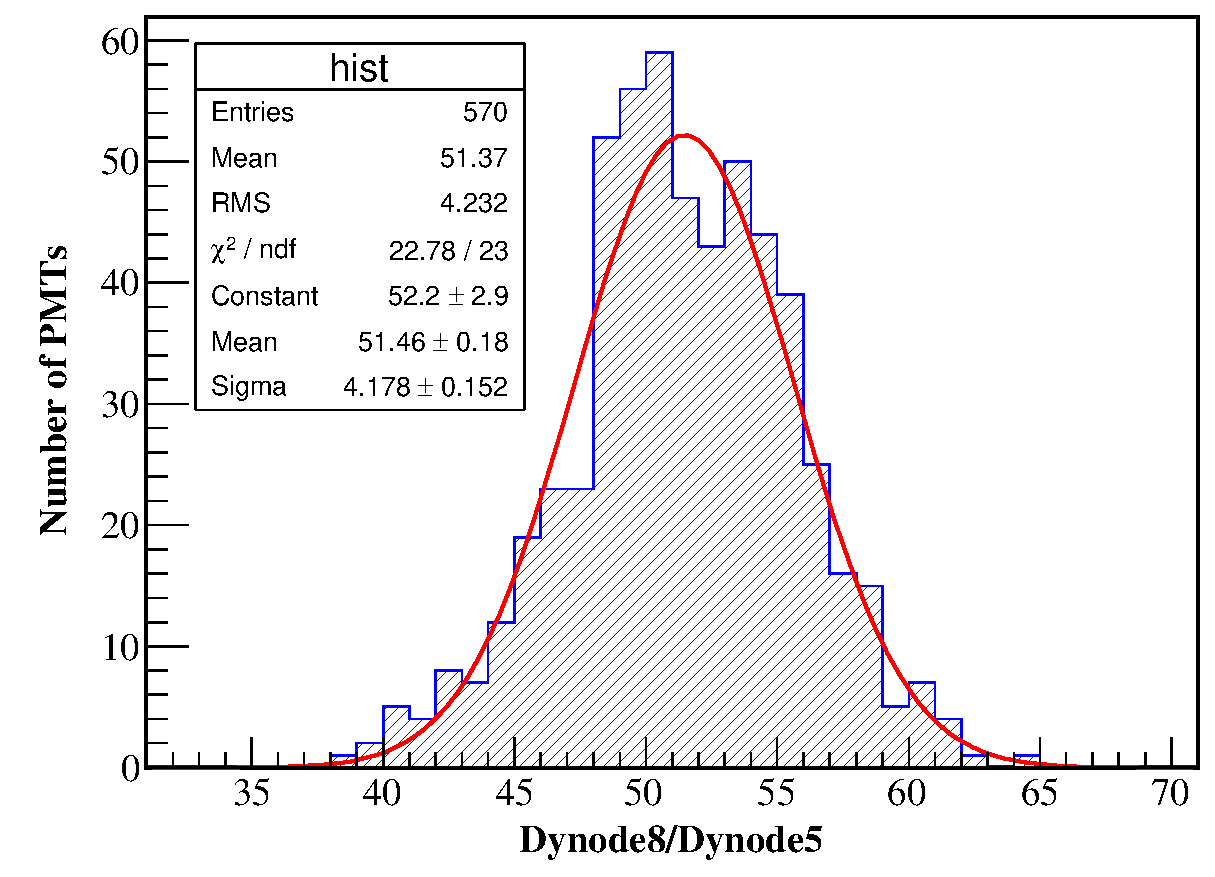
\includegraphics[width=90mm]{dy58_dist}
\caption{Distribution of the Dynode8/Dynode5 at the voltage value equivalent to Hamamastu typical voltage}
\label{fig:dy58_dist}
\end{figure} 

\begin{figure*}[]
 \centering
 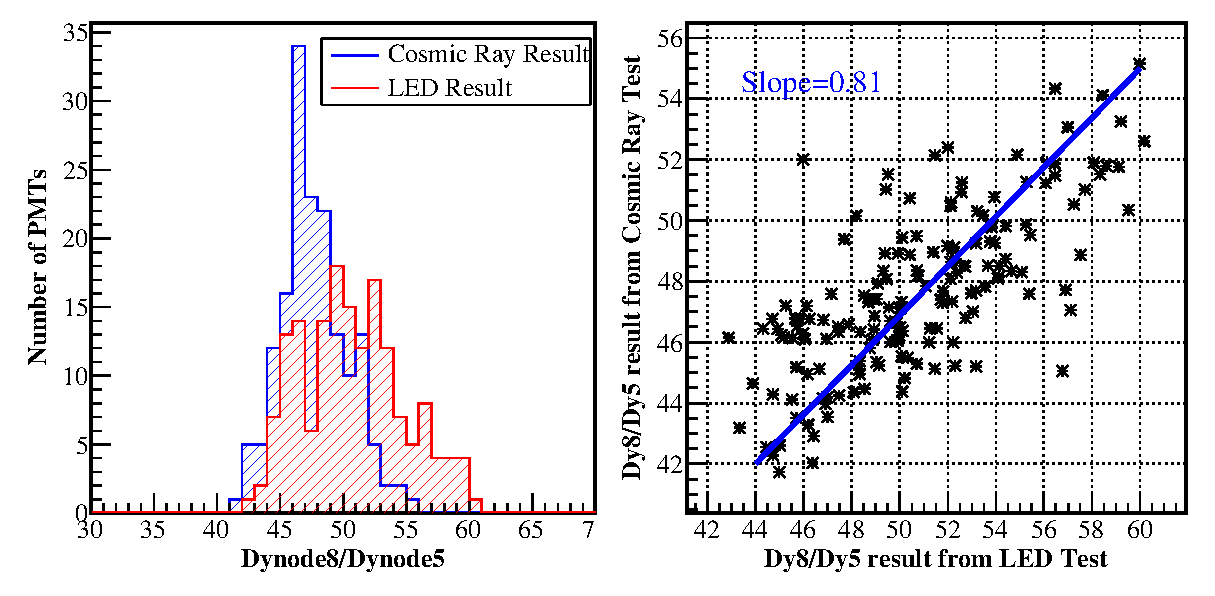
\includegraphics[width=140mm]{dy58_ledvscm}
\caption{Comparison of the dy8/dy5 measured from LED and from cosmic ray.}
\label{fig:dy58_ledvscm}
\end{figure*} 

The ratio between dynode8 and dynode5 is measured by varying the light intensity in a large range until saturation of the dynode 8 is observed(see Fig\ref{fig:dy58_example}).
The same procedure is repeated at 7 voltage steps(700V to 1000V with a 50V step) to get the dependency on voltage.
As with the gain of dynode8, the dependency can be fitted accurately with a power law function, as shown in the inset graph of Fig.\ref{fig:dy58_example}.
The dy8/dy5 ratio can then be calculated at any voltage value based on the fitting result.
As an example, the distribution of dy8/dy5 ratios at the Hamamastu equivalent voltage is shown in Fig.\ref{fig:dy58_dist}.

Matching between the result measured using the test bench in this paper and the result measured from comsic ray after coupling to the scintillator has been checked for a small sample of tubes.
As shown in Fig.\ref{fig:dy58_ledvscm}, a small shift of the mean value exists and the distribution of cosmic ray test is narrower than that of LED test. 
This effect may be attributed to the fact that in cosmic ray test the result is an average of the response in the whole cathode surface, while in LED test the result is the reponse at the center of the cathode surface with a spot of \SI{1}{\milli\meter}.


\subsection{Testing of Cathode Uniformity}
\label{sec:psd_cathodescan}

\begin{figure}[h!]
 \centering
 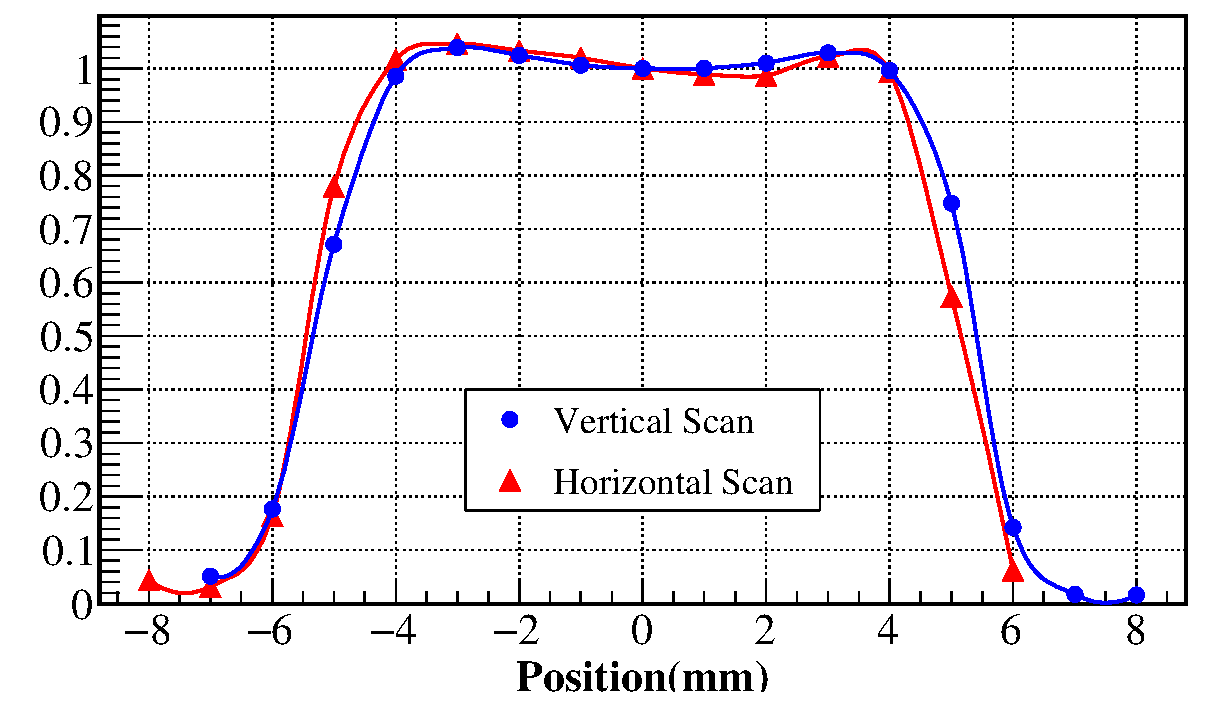
\includegraphics[width=90mm]{cathode_uniformity}
\caption{A typical cathode uniformity}
\label{fig:cathode_uniformity}
\end{figure} 

A \textit{PTVProgram} for cathode uniformity characterization is implemented to validate the position scanning ability of the test bench.
The scanning is performed in the verical and horizontal direction with a step of \SI{1}{\milli\meter}.
At each position, the relative gain is measured according to the method described in Sec.\ref{sec:psd_gain}.

Cathode uniformity of 20 tubes have been measured in a single test run using this \textit{PTVProgram}.
A typical distribution of cathode uniformity is shown in Fig.\ref{fig:cathode_uniformity}.
R4443 Mod2 has a photocathode with a minimum effective area of about \SI{10}{\milli\meter}.
The results of all 20 tubes are summarized and it is found that in the central \SI{9}{\milli\meter} of the photocathode, about \SI{75}{\percent} of the testing data are within \textpm\SI{10}{\percent} range around each tube's average value.

\section{Performance of the test bench}
\label{sec:performance}

Performance of the test bench is extracted from the reference PMTs using the data obtained in the PMT characterization for PSD.

As a first step, stability of the reference PMT configuration is checked.
If stable, the response to various light intensities of the two reference PMTs shall be linearly correlated.
An example is shown in Fig.\ref{fig:refgain_relation}, where the data points can be fitted quite well with linear function.
The slope of the fitting function does not depends on the light intensities used:
\begin{equation}
 M = \frac{G_{ref1} T_{ref1}}{G_{ref2} T_{ref2}}
\end{equation}
where $G_{ref}$ is the absolute gain of each reference PMT and $T_{ref}$ is the transmition difference of fibres between reference channels.
As transmition difference is a fixed parameter(the good linearity of the fitting is an indication of that), $M$ is only related to the gain difference between the reference PMTs.
$M$ values are calculated for all test runs and the variance of it is found to be \SI{0.48}{\percent}.
This result verifies the high stability of the reference PMTs.

By investigating the response of the reference PMT to a fixed light source setting, a maximum variation of \SI{4}{\percent} in the light intensity of LED is observed during a period of about one month.
Light intensity fluctuation can be corrected using the method described in \ref{sec:psd_gain}.
As two reference PMTs exists, this method can be validated by using one of them for light intensity correction and then checking the relative gain of the other. 
As shown in Fig.\ref{fig:led_stability}, after correction the stability of the light source is controlled within \textpm\SI{0.5}{\percent}.

Reference PMTs undergo the same testing procedures as other tubes under test.
Thus, spread of the distribution of the parameters of reference PMT is an indication of the uncertainty of the testing method.
As an example, distribution of dynode8/dynode5 of the reference PMTs is shown in Fig.\ref{fig:dy58_stabiltiy}, where the results from different voltage steps are scaled to their respective mean value of all test runs.
The variance is \SI{1.59}{\percent}, which is adoptted as the testing uncertainty of the dynode8/dynode5 measurement.
%%As an example, dynode8/dynode5 of the reference PMTs at a fixed voltage are first scaled to their mean value of all test runs.
%%Then, scaled value at all voltage steps are filled into the histogram as shown in Fig.\ref{fig:dy58_stabiltiy}.
%%The variance of the distribution is \SI{1.59}{\percent}, which is adoptted as the testing uncertainty of the dynode8/dynode5 measurement.
In the same way, the uncertainty in the measurement of relative gain is estimated to be \SI{0.53}{\percent}. 

\begin{figure}[h!]
 \centering
 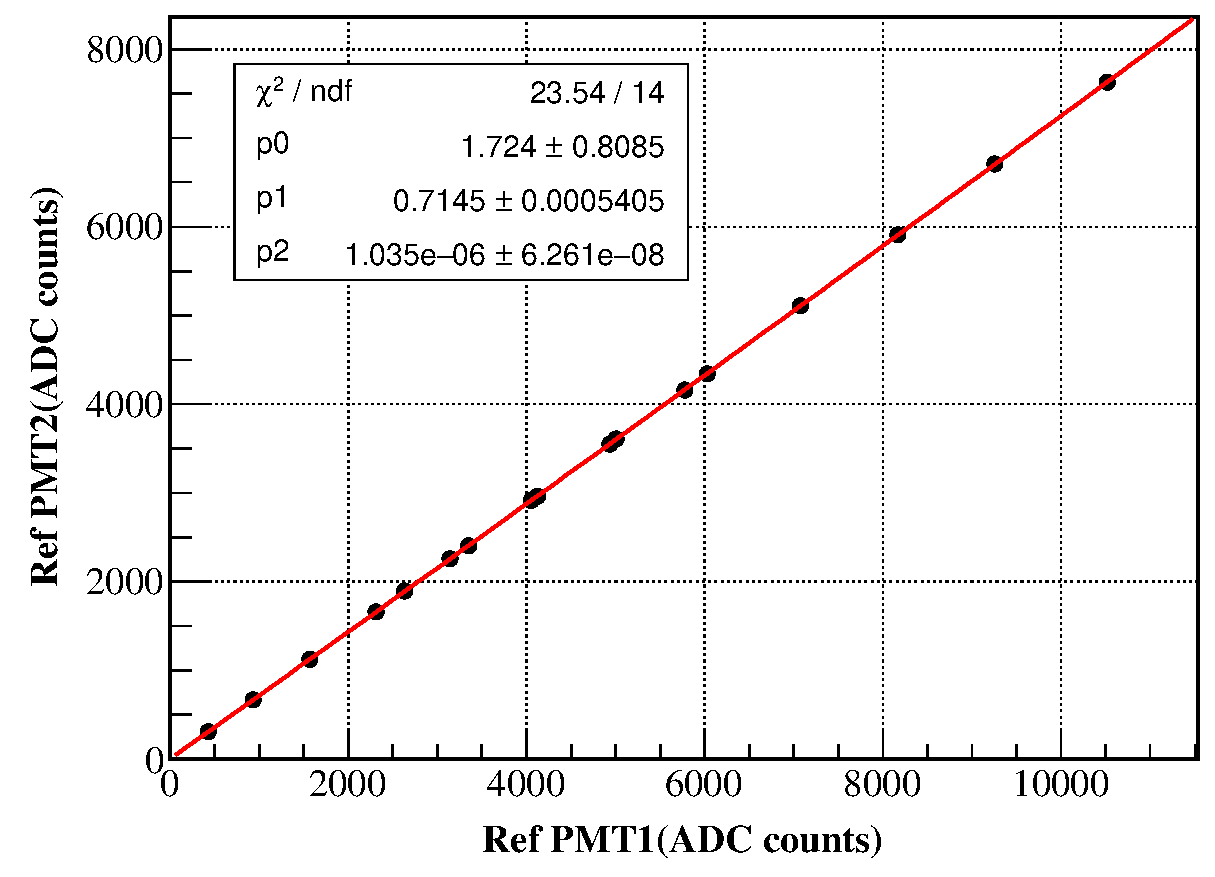
\includegraphics[width=90mm]{RelativeGainRef}
\caption{Example of the correlation between reference PMTs at various light intensities at 1000V.}
\label{fig:refgain_relation}
\end{figure} 

\begin{figure}[h!]
 \centering
 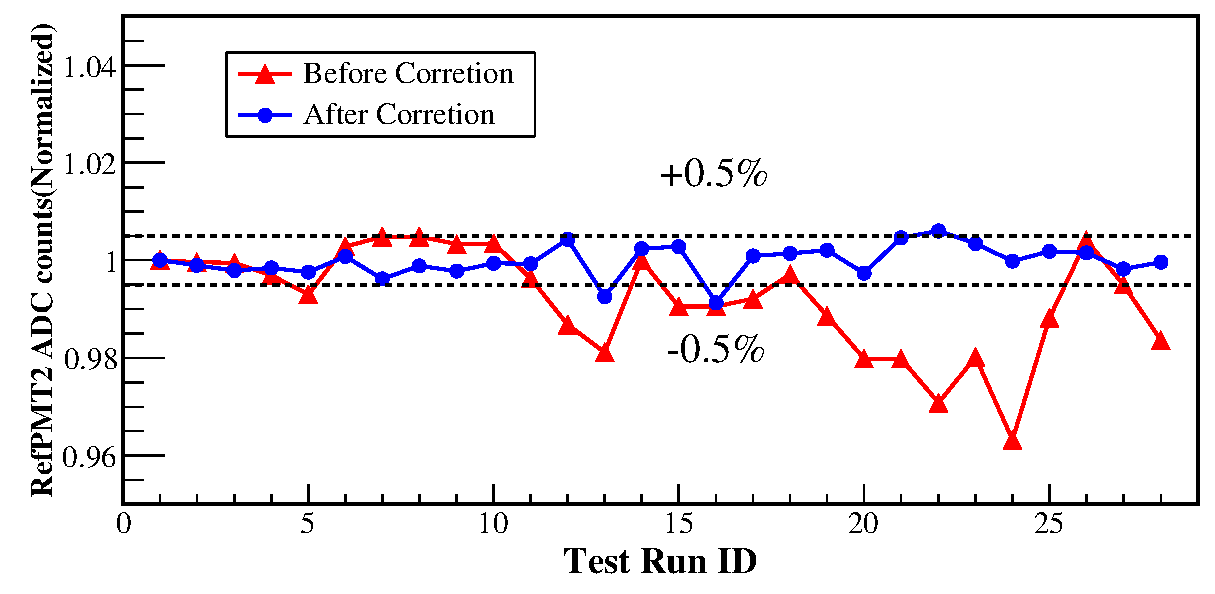
\includegraphics[width=90mm]{led_stability}
\caption{Stability of the light source monitored by reference PMT2.
The data corresponds to a period of about one month and is all scaled to the first test run.
Red line: mean ADC counts response to the same light source setting before light intensity correction.
Blue line: relative gain measured using reference PMT1 for light intensity correction.}
\label{fig:led_stability}
\end{figure} 

\begin{figure}[h!]
 \centering
 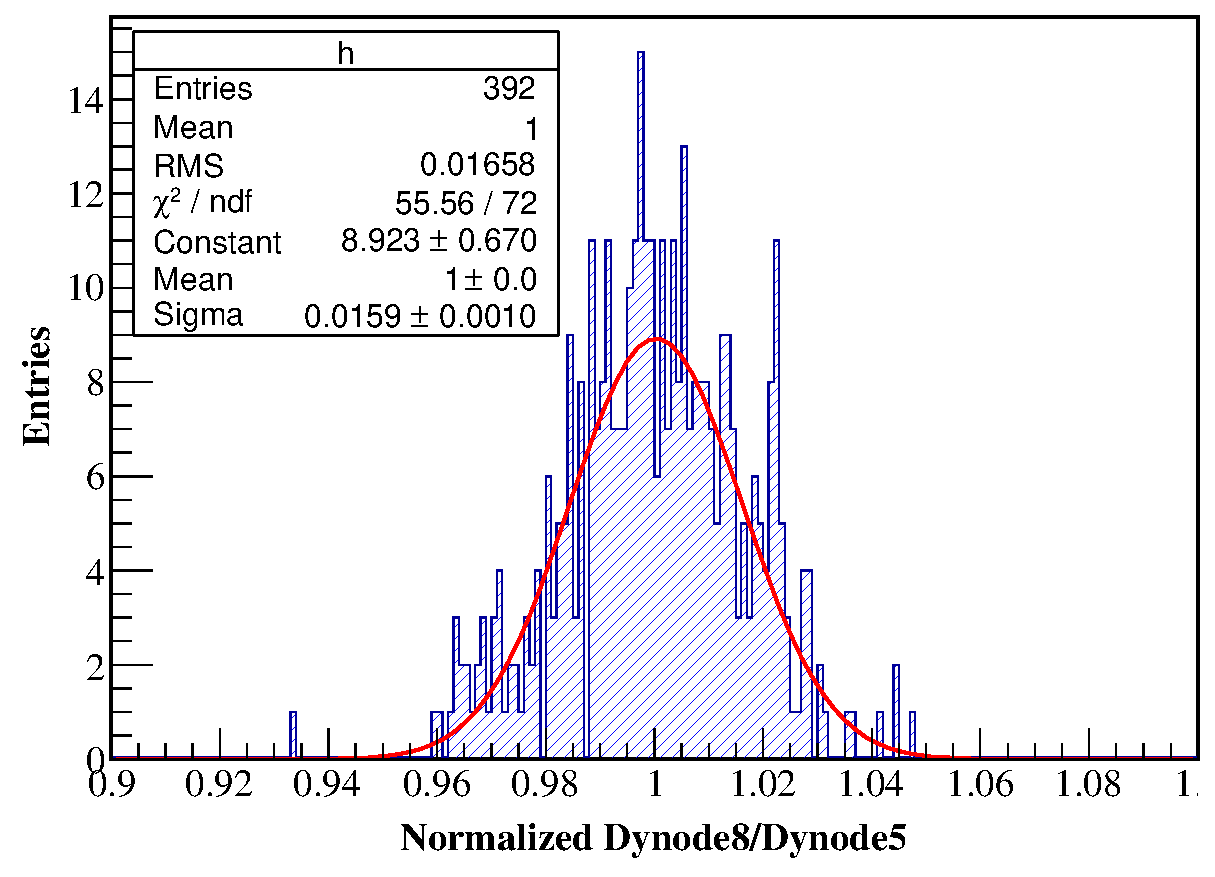
\includegraphics[width=90mm]{RefDy58Dist}
\caption{Distribution of the dynode8/dynode5 ratio of the reference PMTs measured by the test bench.
Results from all voltage steps are scaled to their respective mean value of all test runs.}
\label{fig:dy58_stabiltiy}
\end{figure} 



\begin{comment}
\begin{figure}[h!]
 \centering
 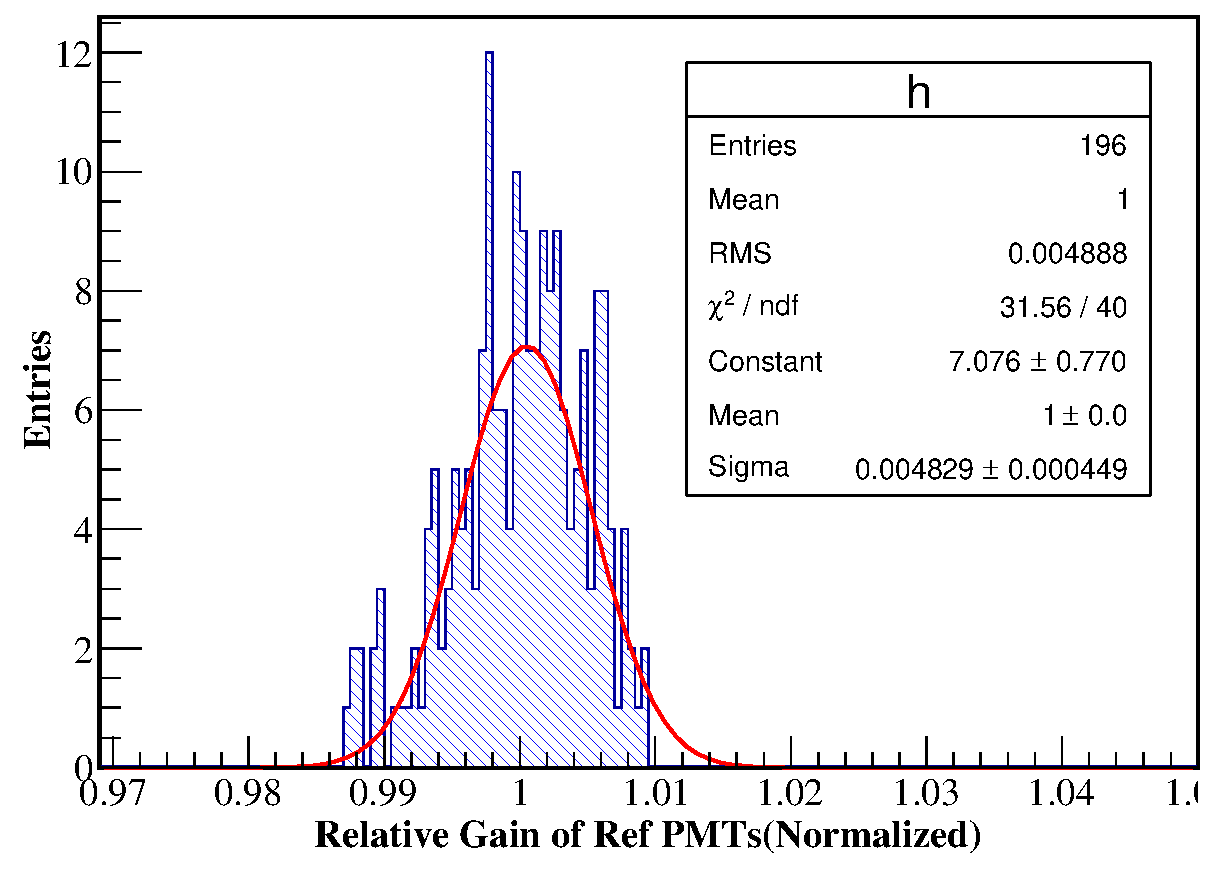
\includegraphics[width=90mm]{RelativeGainRefDist}
\caption{Stability of Gain Measurement}
\label{fig:gain_stability}
\end{figure} 
\end{comment}
%%%%%%%%%%%%%%%%  Conclustion   %%%%%%%%%%%%%%%%%%%%%%%
\section{Conclusions}
\label{sec:conclustions}

%%%%%%%%%%%%%%%% Acknowledgement %%%%%%%%%%%%%%%%%%%%%%%
\section*{Acknowledgement}

This work was supported by the Strategic Priority Research Program on Space Science of the Chinese Academy of Science, Grant No. XDA04040202- 3. 
%%%%%%%%%%%%%%%%    Appendix     %%%%%%%%%%%%%%%%%%%%%%%
%% The Appendices part is started with the command \appendix;
%% appendix sections are then done as normal sections
\appendix
\section{}
\label{app:}

%%%%%%%%%%%%%%%%   Bibliography  %%%%%%%%%%%%%%%%%%%%%%%
%% bibliography style
\section*{References}
\bibliographystyle{elsarticle-num}

%% From BibTex file
\bibliography{mybib}

%% From hand-writing
\begin{comment}
%%\begin{thebibliography}{00}

%%\bibitem{CEBAF12}
%%V.D. Burkert,  \emph{arXiv:1203.2373v1 [nucl-ex]},  2012.

%%\bibitem{CLAS}
%%B.A. Mecking \emph{et al.},  Nucl. Ins. and Meth. in Phys. Research {\bf A503} (2003) 513

%%\end{thebibliography}
\end{comment}

\end{document}
\endinput